\documentclass[a4paper]{book}
\usepackage{makeidx}
\usepackage{graphicx}
\usepackage{multicol}
\usepackage{float}
\usepackage{listings}
\usepackage{color}
\usepackage{ifthen}
\usepackage[table]{xcolor}
\usepackage{textcomp}
\usepackage{alltt}
\usepackage{ifpdf}
\ifpdf
\usepackage[pdftex,
            pagebackref=true,
            colorlinks=true,
            linkcolor=blue,
            unicode
           ]{hyperref}
\else
\usepackage[ps2pdf,
            pagebackref=true,
            colorlinks=true,
            linkcolor=blue,
            unicode
           ]{hyperref}
\usepackage{pspicture}
\fi
\usepackage[utf8]{inputenc}
\usepackage{mathptmx}
\usepackage[scaled=.90]{helvet}
\usepackage{courier}
\usepackage{sectsty}
\usepackage[titles]{tocloft}
\usepackage{doxygen}
\lstset{language=C++,inputencoding=utf8,basicstyle=\footnotesize,breaklines=true,breakatwhitespace=true,tabsize=8,numbers=left }
\makeindex
\setcounter{tocdepth}{3}
\renewcommand{\footrulewidth}{0.4pt}
\renewcommand{\familydefault}{\sfdefault}
\begin{document}
\hypersetup{pageanchor=false}
\begin{titlepage}
\vspace*{7cm}
\begin{center}
{\Large Reference Manual}\\
\vspace*{1cm}
{\large Generated by Doxygen 1.7.4}\\
\vspace*{0.5cm}
{\small Thu Aug 9 2012 12:22:40}\\
\end{center}
\end{titlepage}
\clearemptydoublepage
\pagenumbering{roman}
\tableofcontents
\clearemptydoublepage
\pagenumbering{arabic}
\hypersetup{pageanchor=true}
\chapter{Class Index}
\section{Class Hierarchy}
This inheritance list is sorted roughly, but not completely, alphabetically:\begin{DoxyCompactList}
\item \contentsline{section}{CatmullRomBlend$<$ real, dim $>$}{\pageref{classCatmullRomBlend}}{}
\item \contentsline{section}{PolygonalCurve$<$ real, dim, Point, Vector $>$::DPitem}{\pageref{structPolygonalCurve_1_1DPitem}}{}
\item \contentsline{section}{PolygonalCurve$<$ real, dim, Point, Vector $>$}{\pageref{classPolygonalCurve}}{}
\item \contentsline{section}{VectorN$<$ real, dim $>$}{\pageref{classVectorN}}{}
\begin{DoxyCompactList}
\item \contentsline{section}{PointN$<$ real, dim $>$}{\pageref{classPointN}}{}
\end{DoxyCompactList}
\end{DoxyCompactList}

\chapter{Class Index}
\section{Class List}
Here are the classes, structs, unions and interfaces with brief descriptions:\begin{DoxyCompactList}
\item\contentsline{section}{\hyperlink{classCatmullRomBlend}{CatmullRomBlend$<$ real, dim $>$} }{\pageref{classCatmullRomBlend}}{}
\item\contentsline{section}{\hyperlink{structPolygonalCurve_1_1DPitem}{PolygonalCurve$<$ real, dim, Point, Vector $>$::DPitem} (Class used by the douglasPeuckerRank method )}{\pageref{structPolygonalCurve_1_1DPitem}}{}
\item\contentsline{section}{\hyperlink{classPointN}{PointN$<$ real, dim $>$} }{\pageref{classPointN}}{}
\item\contentsline{section}{\hyperlink{classPolygonalCurve}{PolygonalCurve$<$ real, dim, Point, Vector $>$} (N-\/dimensional polygonal chain )}{\pageref{classPolygonalCurve}}{}
\item\contentsline{section}{\hyperlink{classVectorN}{VectorN$<$ real, dim $>$} (A N-\/dimensional Vector class )}{\pageref{classVectorN}}{}
\end{DoxyCompactList}

\chapter{Class Documentation}
\hypertarget{classCatmullRomBlend}{
\section{CatmullRomBlend$<$ real, dim $>$ Class Template Reference}
\label{classCatmullRomBlend}\index{CatmullRomBlend@{CatmullRomBlend}}
}


{\ttfamily \#include $<$catmullrom.hpp$>$}

\subsection*{Public Member Functions}
\begin{DoxyCompactItemize}
\item 
\hyperlink{classCatmullRomBlend_aa6064a7b7c7ce3ad80485c31f1d24142}{CatmullRomBlend} (real tension=0.5)
\begin{DoxyCompactList}\small\item\em Constructor. \end{DoxyCompactList}\item 
void \hyperlink{classCatmullRomBlend_a56e328baf4beb49e924d847ba727edce}{blendFactors} (real u, real factor\mbox{[}$\,$\mbox{]}) const 
\begin{DoxyCompactList}\small\item\em Given a parameter u, computes the blending factors for the four control points. \end{DoxyCompactList}\item 
void \hyperlink{classCatmullRomBlend_a7ec31af121c83ccf2f8a6a42d79b51fa}{blendPoint} (real u, const real p0\mbox{[}$\,$\mbox{]}, const real p1\mbox{[}$\,$\mbox{]}, const real p2\mbox{[}$\,$\mbox{]}, const real p3\mbox{[}$\,$\mbox{]}, real p\mbox{[}$\,$\mbox{]}) const 
\begin{DoxyCompactList}\small\item\em Given a parameter u and the coordinates of 4 control points, returns computes the interpolated point. \end{DoxyCompactList}\end{DoxyCompactItemize}
\subsection*{Protected Attributes}
\begin{DoxyCompactItemize}
\item 
\hypertarget{classCatmullRomBlend_a8a694bbc355517f628c36c3a52c9e48a}{
real \hyperlink{classCatmullRomBlend_a8a694bbc355517f628c36c3a52c9e48a}{tau}}
\label{classCatmullRomBlend_a8a694bbc355517f628c36c3a52c9e48a}

\begin{DoxyCompactList}\small\item\em Tension. \end{DoxyCompactList}\end{DoxyCompactItemize}


\subsection{Detailed Description}
\subsubsection*{template$<$typename real, unsigned int dim = 3$>$class CatmullRomBlend$<$ real, dim $>$}

Cubic Catmull-\/Rom Interpolator.


\begin{DoxyParams}{Parameters}
{\em real,:} & scalar type to use (usually float or double) \\
\hline
{\em dim,:} & domain dimension \\
\hline
\end{DoxyParams}


\subsection{Constructor \& Destructor Documentation}
\hypertarget{classCatmullRomBlend_aa6064a7b7c7ce3ad80485c31f1d24142}{
\index{CatmullRomBlend@{CatmullRomBlend}!CatmullRomBlend@{CatmullRomBlend}}
\index{CatmullRomBlend@{CatmullRomBlend}!CatmullRomBlend@{CatmullRomBlend}}
\subsubsection[{CatmullRomBlend}]{\setlength{\rightskip}{0pt plus 5cm}template$<$typename real, unsigned int dim = 3$>$ {\bf CatmullRomBlend}$<$ real, dim $>$::{\bf CatmullRomBlend} (
\begin{DoxyParamCaption}
\item[{real}]{tension = {\ttfamily 0.5}}
\end{DoxyParamCaption}
)\hspace{0.3cm}{\ttfamily  \mbox{[}inline\mbox{]}}}}
\label{classCatmullRomBlend_aa6064a7b7c7ce3ad80485c31f1d24142}


Constructor. 


\begin{DoxyParams}{Parameters}
{\em tension,:} & the tension. \\
\hline
\end{DoxyParams}


\subsection{Member Function Documentation}
\hypertarget{classCatmullRomBlend_a56e328baf4beb49e924d847ba727edce}{
\index{CatmullRomBlend@{CatmullRomBlend}!blendFactors@{blendFactors}}
\index{blendFactors@{blendFactors}!CatmullRomBlend@{CatmullRomBlend}}
\subsubsection[{blendFactors}]{\setlength{\rightskip}{0pt plus 5cm}template$<$typename real, unsigned int dim = 3$>$ void {\bf CatmullRomBlend}$<$ real, dim $>$::blendFactors (
\begin{DoxyParamCaption}
\item[{real}]{u, }
\item[{real}]{factor\mbox{[}$\,$\mbox{]}}
\end{DoxyParamCaption}
) const\hspace{0.3cm}{\ttfamily  \mbox{[}inline\mbox{]}}}}
\label{classCatmullRomBlend_a56e328baf4beb49e924d847ba727edce}


Given a parameter u, computes the blending factors for the four control points. 


\begin{DoxyParams}{Parameters}
{\em u,:} & curve parameter. \\
\hline
{\em factor} & (output): array of 4 blending factors. \\
\hline
\end{DoxyParams}
\hypertarget{classCatmullRomBlend_a7ec31af121c83ccf2f8a6a42d79b51fa}{
\index{CatmullRomBlend@{CatmullRomBlend}!blendPoint@{blendPoint}}
\index{blendPoint@{blendPoint}!CatmullRomBlend@{CatmullRomBlend}}
\subsubsection[{blendPoint}]{\setlength{\rightskip}{0pt plus 5cm}template$<$typename real, unsigned int dim = 3$>$ void {\bf CatmullRomBlend}$<$ real, dim $>$::blendPoint (
\begin{DoxyParamCaption}
\item[{real}]{u, }
\item[{const real}]{p0\mbox{[}$\,$\mbox{]}, }
\item[{const real}]{p1\mbox{[}$\,$\mbox{]}, }
\item[{const real}]{p2\mbox{[}$\,$\mbox{]}, }
\item[{const real}]{p3\mbox{[}$\,$\mbox{]}, }
\item[{real}]{p\mbox{[}$\,$\mbox{]}}
\end{DoxyParamCaption}
) const\hspace{0.3cm}{\ttfamily  \mbox{[}inline\mbox{]}}}}
\label{classCatmullRomBlend_a7ec31af121c83ccf2f8a6a42d79b51fa}


Given a parameter u and the coordinates of 4 control points, returns computes the interpolated point. 


\begin{DoxyParams}{Parameters}
{\em u,:} & curve parameter. \\
\hline
{\em p0,:} & first control point (at least size dim). \\
\hline
{\em p1,:} & second control point (at least size dim). \\
\hline
{\em p2,:} & third control point (at least size dim). \\
\hline
{\em p3,:} & fourth control point (at least size dim). \\
\hline
{\em p} & (output): interpolated point. \\
\hline
\end{DoxyParams}


The documentation for this class was generated from the following file:\begin{DoxyCompactItemize}
\item 
catmullrom.hpp\end{DoxyCompactItemize}

\hypertarget{structPolygonalCurve_1_1DPitem}{
\section{PolygonalCurve$<$ real, dim, Point, Vector $>$::DPitem Struct Reference}
\label{structPolygonalCurve_1_1DPitem}\index{PolygonalCurve::DPitem@{PolygonalCurve::DPitem}}
}


class used by the douglasPeuckerRank method.  




{\ttfamily \#include $<$curven.hpp$>$}

\subsection*{Public Member Functions}
\begin{DoxyCompactItemize}
\item 
\hyperlink{structPolygonalCurve_1_1DPitem_a7bc8e2684372da099f75ed38e064d948}{DPitem} (unsigned f, unsigned l, const \hyperlink{classPolygonalCurve}{PolygonalCurve}$<$ real, dim, Point, Vector $>$ \&poly)
\begin{DoxyCompactList}\small\item\em Constructor. \end{DoxyCompactList}\item 
\hypertarget{structPolygonalCurve_1_1DPitem_a55d33e0b8ae80e9ac78d7f2861e64b20}{
bool \hyperlink{structPolygonalCurve_1_1DPitem_a55d33e0b8ae80e9ac78d7f2861e64b20}{operator$<$} (const \hyperlink{structPolygonalCurve_1_1DPitem}{DPitem} \&other) const }
\label{structPolygonalCurve_1_1DPitem_a55d33e0b8ae80e9ac78d7f2861e64b20}

\begin{DoxyCompactList}\small\item\em Operator $<$. \end{DoxyCompactList}\end{DoxyCompactItemize}
\subsection*{Public Attributes}
\begin{DoxyCompactItemize}
\item 
\hypertarget{structPolygonalCurve_1_1DPitem_af53f3be5120386c8df25c6ff2283d2e9}{
unsigned \hyperlink{structPolygonalCurve_1_1DPitem_af53f3be5120386c8df25c6ff2283d2e9}{first}}
\label{structPolygonalCurve_1_1DPitem_af53f3be5120386c8df25c6ff2283d2e9}

\begin{DoxyCompactList}\small\item\em index of the first vertex of the range \end{DoxyCompactList}\item 
\hypertarget{structPolygonalCurve_1_1DPitem_ad13567bd2031902289e8ff928a227a95}{
unsigned \hyperlink{structPolygonalCurve_1_1DPitem_ad13567bd2031902289e8ff928a227a95}{last}}
\label{structPolygonalCurve_1_1DPitem_ad13567bd2031902289e8ff928a227a95}

\begin{DoxyCompactList}\small\item\em index of the last vertex of the range \end{DoxyCompactList}\item 
unsigned \hyperlink{structPolygonalCurve_1_1DPitem_a08cfeb2a6ec60cab38547705e132e36c}{farthest}
\item 
\hypertarget{structPolygonalCurve_1_1DPitem_a7d29594a956d56a171f48f6d3251fd2c}{
double \hyperlink{structPolygonalCurve_1_1DPitem_a7d29594a956d56a171f48f6d3251fd2c}{dist}}
\label{structPolygonalCurve_1_1DPitem_a7d29594a956d56a171f48f6d3251fd2c}

\begin{DoxyCompactList}\small\item\em squared perpendicular distance from the line segment \end{DoxyCompactList}\end{DoxyCompactItemize}


\subsection{Detailed Description}
\subsubsection*{template$<$typename real, unsigned int dim, class Point = PointN$<$real,dim$>$, class Vector = VectorN$<$real,dim$>$$>$struct PolygonalCurve$<$ real, dim, Point, Vector $>$::DPitem}

class used by the douglasPeuckerRank method. 

This is used as an element in the priority queue needed by the douglasPeuckerRank method. 

\subsection{Constructor \& Destructor Documentation}
\hypertarget{structPolygonalCurve_1_1DPitem_a7bc8e2684372da099f75ed38e064d948}{
\index{PolygonalCurve::DPitem@{PolygonalCurve::DPitem}!DPitem@{DPitem}}
\index{DPitem@{DPitem}!PolygonalCurve::DPitem@{PolygonalCurve::DPitem}}
\subsubsection[{DPitem}]{\setlength{\rightskip}{0pt plus 5cm}template$<$typename real, unsigned int dim, class Point = PointN$<$real,dim$>$, class Vector = VectorN$<$real,dim$>$$>$ {\bf PolygonalCurve}$<$ real, dim, Point, Vector $>$::DPitem::DPitem (
\begin{DoxyParamCaption}
\item[{unsigned}]{f, }
\item[{unsigned}]{l, }
\item[{const {\bf PolygonalCurve}$<$ real, dim, Point, Vector $>$ \&}]{poly}
\end{DoxyParamCaption}
)\hspace{0.3cm}{\ttfamily  \mbox{[}inline\mbox{]}}}}
\label{structPolygonalCurve_1_1DPitem_a7bc8e2684372da099f75ed38e064d948}


Constructor. 

Builds an item corresponding to the a vertex range of a polygonal curve.


\begin{DoxyParams}{Parameters}
{\em f} & index of first point in poly \\
\hline
{\em l} & index of last point in poly \\
\hline
{\em poly} & polygonal curve which is being generalized \\
\hline
\end{DoxyParams}


\subsection{Member Data Documentation}
\hypertarget{structPolygonalCurve_1_1DPitem_a08cfeb2a6ec60cab38547705e132e36c}{
\index{PolygonalCurve::DPitem@{PolygonalCurve::DPitem}!farthest@{farthest}}
\index{farthest@{farthest}!PolygonalCurve::DPitem@{PolygonalCurve::DPitem}}
\subsubsection[{farthest}]{\setlength{\rightskip}{0pt plus 5cm}template$<$typename real, unsigned int dim, class Point = PointN$<$real,dim$>$, class Vector = VectorN$<$real,dim$>$$>$ unsigned {\bf PolygonalCurve}$<$ real, dim, Point, Vector $>$::{\bf DPitem::farthest}}}
\label{structPolygonalCurve_1_1DPitem_a08cfeb2a6ec60cab38547705e132e36c}
index between first and last which is farthest from the line segment defined by the vertices first and last 

The documentation for this struct was generated from the following file:\begin{DoxyCompactItemize}
\item 
curven.hpp\end{DoxyCompactItemize}

\hypertarget{classPointN}{
\section{PointN$<$ real, dim $>$ Class Template Reference}
\label{classPointN}\index{PointN@{PointN}}
}


{\ttfamily \#include $<$vectorn.hpp$>$}

Inheritance diagram for PointN$<$ real, dim $>$:\begin{figure}[H]
\begin{center}
\leavevmode
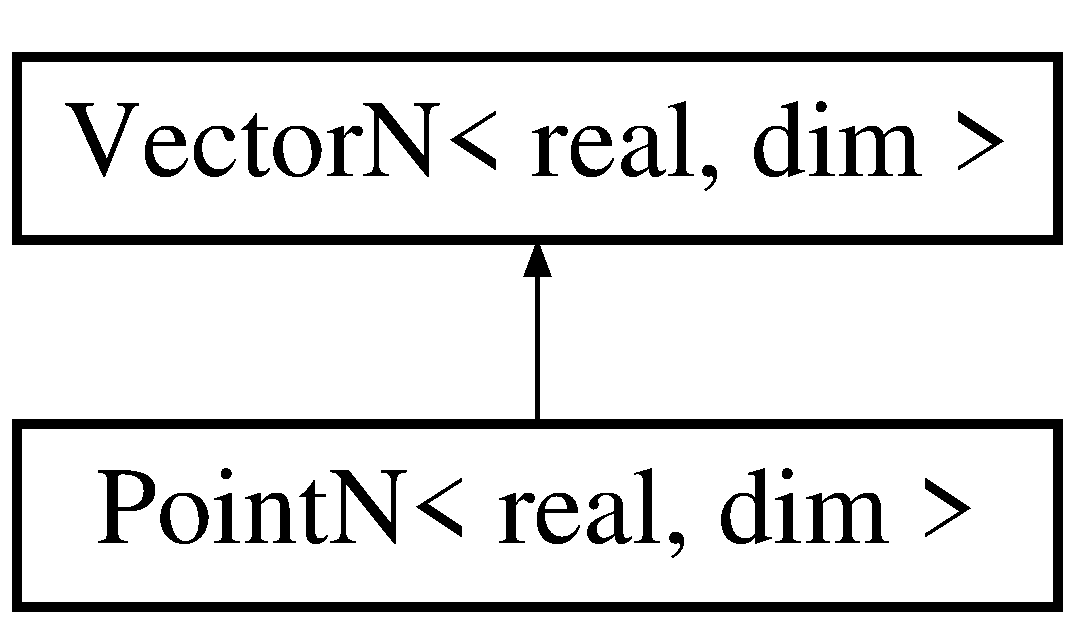
\includegraphics[height=2.000000cm]{classPointN}
\end{center}
\end{figure}
\subsection*{Public Member Functions}
\begin{DoxyCompactItemize}
\item 
\hypertarget{classPointN_aeecdfb6e7bc275830b3910790a12d30c}{
\hyperlink{classPointN_aeecdfb6e7bc275830b3910790a12d30c}{PointN} ()}
\label{classPointN_aeecdfb6e7bc275830b3910790a12d30c}

\begin{DoxyCompactList}\small\item\em Empty constructor. \end{DoxyCompactList}\item 
\hypertarget{classPointN_a47ac5553535eb3ddf9a23fd9b2d18211}{
\hyperlink{classPointN_a47ac5553535eb3ddf9a23fd9b2d18211}{PointN} (const real v\mbox{[}$\,$\mbox{]})}
\label{classPointN_a47ac5553535eb3ddf9a23fd9b2d18211}

\begin{DoxyCompactList}\small\item\em Constructor from an array of coordinates. \end{DoxyCompactList}\item 
\hypertarget{classPointN_acdcac068cc838de9c2dd029c044d0cd3}{
\hyperlink{classPointN_acdcac068cc838de9c2dd029c044d0cd3}{PointN} (const \hyperlink{classVectorN}{VectorN}$<$ real, dim $>$ \&v)}
\label{classPointN_acdcac068cc838de9c2dd029c044d0cd3}

\begin{DoxyCompactList}\small\item\em Constructor from another \hyperlink{classVectorN}{VectorN}. \end{DoxyCompactList}\item 
\hypertarget{classPointN_a538c649af189bd38f47439f074a1b8ae}{
\hyperlink{classPointN_a538c649af189bd38f47439f074a1b8ae}{PointN} (const real v)}
\label{classPointN_a538c649af189bd38f47439f074a1b8ae}

\begin{DoxyCompactList}\small\item\em Constructor from a single coordinate. \end{DoxyCompactList}\item 
\hypertarget{classPointN_a18910c42eb7fc98373fcc45f3c87a6c7}{
\hyperlink{classPointN_a18910c42eb7fc98373fcc45f3c87a6c7}{PointN} (const real x, const real y)}
\label{classPointN_a18910c42eb7fc98373fcc45f3c87a6c7}

\begin{DoxyCompactList}\small\item\em Constructor from two coordinates -\/ must be bidimensional. \end{DoxyCompactList}\item 
\hypertarget{classPointN_a5c33cc8cc3b1071ad6beff66aaf921f2}{
\hyperlink{classPointN_a5c33cc8cc3b1071ad6beff66aaf921f2}{PointN} (const real x, const real y, const real z)}
\label{classPointN_a5c33cc8cc3b1071ad6beff66aaf921f2}

\begin{DoxyCompactList}\small\item\em Constructor from three coordinates -\/ must be tridimensional. \end{DoxyCompactList}\item 
void \hyperlink{classPointN_a98e37e58efb5fdf4f22f38a1eb829ee7}{set} (const \hyperlink{classVectorN}{VectorN}$<$ real, dim $>$ \&v)
\begin{DoxyCompactList}\small\item\em Set coordinates from a vector. \end{DoxyCompactList}\item 
\hypertarget{classPointN_a72bcd72a37795c4a878f69726425d211}{
\hyperlink{classVectorN}{VectorN}$<$ real, dim $>$ \hyperlink{classPointN_a72bcd72a37795c4a878f69726425d211}{toVector} (void)}
\label{classPointN_a72bcd72a37795c4a878f69726425d211}

\begin{DoxyCompactList}\small\item\em Casting to Vector. \end{DoxyCompactList}\item 
\hypertarget{classPointN_a656e5ab6b347867766ef31cda1870827}{
\hyperlink{classPointN}{PointN}$<$ real, dim $>$ \hyperlink{classPointN_a656e5ab6b347867766ef31cda1870827}{affineSum} (real alpha, const \hyperlink{classPointN}{PointN}$<$ real, dim $>$ \&p) const }
\label{classPointN_a656e5ab6b347867766ef31cda1870827}

\begin{DoxyCompactList}\small\item\em Affine multiplication by a scalar. \end{DoxyCompactList}\item 
\hyperlink{classPointN}{PointN}$<$ real, dim $>$ \hyperlink{classPointN_ad05e2c5bba8051980b02914ddaa6c491}{min} (const \hyperlink{classPointN}{PointN}$<$ real, dim $>$ \&p) const 
\begin{DoxyCompactList}\small\item\em Get point with minimum coordinates. \end{DoxyCompactList}\item 
\hyperlink{classPointN}{PointN}$<$ real, dim $>$ \hyperlink{classPointN_acde205e882ffba5dc3cd7000aa7d72b9}{max} (const \hyperlink{classPointN}{PointN}$<$ real, dim $>$ \&p) const 
\begin{DoxyCompactList}\small\item\em Get point with maximum coordinates. \end{DoxyCompactList}\item 
\hypertarget{classPointN_a245fdcfea715eb96303ad5f548881253}{
real \hyperlink{classPointN_a245fdcfea715eb96303ad5f548881253}{dist2} (const \hyperlink{classPointN}{PointN}$<$ real, dim $>$ \&p) const }
\label{classPointN_a245fdcfea715eb96303ad5f548881253}

\begin{DoxyCompactList}\small\item\em Squared distance between two points. \end{DoxyCompactList}\item 
\hypertarget{classPointN_ac82ba1c6569d98244a1128f47e8aa9b7}{
real \hyperlink{classPointN_ac82ba1c6569d98244a1128f47e8aa9b7}{dist} (const \hyperlink{classPointN}{PointN}$<$ real, dim $>$ \&p) const }
\label{classPointN_ac82ba1c6569d98244a1128f47e8aa9b7}

\begin{DoxyCompactList}\small\item\em Euclidian distance between two points. \end{DoxyCompactList}\end{DoxyCompactItemize}


\subsection{Detailed Description}
\subsubsection*{template$<$typename real = double, unsigned int dim = 3$>$class PointN$<$ real, dim $>$}

A N-\/dimensional Point class 

\subsection{Member Function Documentation}
\hypertarget{classPointN_acde205e882ffba5dc3cd7000aa7d72b9}{
\index{PointN@{PointN}!max@{max}}
\index{max@{max}!PointN@{PointN}}
\subsubsection[{max}]{\setlength{\rightskip}{0pt plus 5cm}template$<$typename real = double, unsigned int dim = 3$>$ {\bf PointN}$<$real,dim$>$ {\bf PointN}$<$ real, dim $>$::max (
\begin{DoxyParamCaption}
\item[{const {\bf PointN}$<$ real, dim $>$ \&}]{p}
\end{DoxyParamCaption}
) const\hspace{0.3cm}{\ttfamily  \mbox{[}inline\mbox{]}}}}
\label{classPointN_acde205e882ffba5dc3cd7000aa7d72b9}


Get point with maximum coordinates. 


\begin{DoxyParams}{Parameters}
{\em p} & another point. \\
\hline
\end{DoxyParams}
\begin{DoxyReturn}{Returns}
point whose coordinates are the maximum between this point's coordinates and p's 
\end{DoxyReturn}
\hypertarget{classPointN_ad05e2c5bba8051980b02914ddaa6c491}{
\index{PointN@{PointN}!min@{min}}
\index{min@{min}!PointN@{PointN}}
\subsubsection[{min}]{\setlength{\rightskip}{0pt plus 5cm}template$<$typename real = double, unsigned int dim = 3$>$ {\bf PointN}$<$real,dim$>$ {\bf PointN}$<$ real, dim $>$::min (
\begin{DoxyParamCaption}
\item[{const {\bf PointN}$<$ real, dim $>$ \&}]{p}
\end{DoxyParamCaption}
) const\hspace{0.3cm}{\ttfamily  \mbox{[}inline\mbox{]}}}}
\label{classPointN_ad05e2c5bba8051980b02914ddaa6c491}


Get point with minimum coordinates. 


\begin{DoxyParams}{Parameters}
{\em p} & another point. \\
\hline
\end{DoxyParams}
\begin{DoxyReturn}{Returns}
point whose coordinates are the minimum between this point's coordinates and p's 
\end{DoxyReturn}
\hypertarget{classPointN_a98e37e58efb5fdf4f22f38a1eb829ee7}{
\index{PointN@{PointN}!set@{set}}
\index{set@{set}!PointN@{PointN}}
\subsubsection[{set}]{\setlength{\rightskip}{0pt plus 5cm}template$<$typename real = double, unsigned int dim = 3$>$ void {\bf PointN}$<$ real, dim $>$::set (
\begin{DoxyParamCaption}
\item[{const {\bf VectorN}$<$ real, dim $>$ \&}]{v}
\end{DoxyParamCaption}
)\hspace{0.3cm}{\ttfamily  \mbox{[}inline\mbox{]}}}}
\label{classPointN_a98e37e58efb5fdf4f22f38a1eb829ee7}


Set coordinates from a vector. 


\begin{DoxyParams}{Parameters}
{\em v,:} & a vector \\
\hline
\end{DoxyParams}


The documentation for this class was generated from the following file:\begin{DoxyCompactItemize}
\item 
vectorn.hpp\end{DoxyCompactItemize}

\hypertarget{classPolygonalCurve}{
\section{PolygonalCurve$<$ real, dim, Point, Vector $>$ Class Template Reference}
\label{classPolygonalCurve}\index{PolygonalCurve@{PolygonalCurve}}
}


N-\/dimensional polygonal chain.  




{\ttfamily \#include $<$curven.hpp$>$}

\subsection*{Classes}
\begin{DoxyCompactItemize}
\item 
struct \hyperlink{structPolygonalCurve_1_1DPitem}{DPitem}
\begin{DoxyCompactList}\small\item\em class used by the douglasPeuckerRank method. \end{DoxyCompactList}\end{DoxyCompactItemize}
\subsection*{Public Member Functions}
\begin{DoxyCompactItemize}
\item 
\hypertarget{classPolygonalCurve_ad49440d5abf4e7d611a08199614946f6}{
\hyperlink{classPolygonalCurve_ad49440d5abf4e7d611a08199614946f6}{PolygonalCurve} (void)}
\label{classPolygonalCurve_ad49440d5abf4e7d611a08199614946f6}

\begin{DoxyCompactList}\small\item\em Empty constructor -\/ builds an open polygonal line with 0 vertices. \end{DoxyCompactList}\item 
\hyperlink{classPolygonalCurve_a765f9ed20f08082f9472163690e3626d}{PolygonalCurve} (const \hyperlink{classPolygonalCurve}{PolygonalCurve}$<$ real, dim, Point, Vector $>$ \&curve)
\begin{DoxyCompactList}\small\item\em Copy constructor. \end{DoxyCompactList}\item 
\hyperlink{classPolygonalCurve_aafe300222bd47264321282b3ff4a1df5}{PolygonalCurve} (const std::vector$<$ Point $>$ \&points)
\begin{DoxyCompactList}\small\item\em Constructor from an array. \end{DoxyCompactList}\item 
virtual void \hyperlink{classPolygonalCurve_a3613ee4e2236f63c266e2366c4c28dd2}{copy} (const \hyperlink{classPolygonalCurve}{PolygonalCurve}$<$ real, dim, Point, Vector $>$ \&curve)
\begin{DoxyCompactList}\small\item\em Copy helper method. \end{DoxyCompactList}\item 
virtual \hyperlink{classPolygonalCurve}{PolygonalCurve} \& \hyperlink{classPolygonalCurve_ac7a5c51ecf180237723091daa1265f1b}{operator=} (const \hyperlink{classPolygonalCurve}{PolygonalCurve}$<$ real, dim, Point, Vector $>$ \&curve)
\begin{DoxyCompactList}\small\item\em Assignment operator. \end{DoxyCompactList}\item 
virtual Point \& \hyperlink{classPolygonalCurve_a46374e7c2d60d51f504cd949ef691abb}{operator\mbox{[}$\,$\mbox{]}} (unsigned i)
\begin{DoxyCompactList}\small\item\em Indexing operator. \end{DoxyCompactList}\item 
virtual Point \hyperlink{classPolygonalCurve_a993101c839429b2fb6ba4cf487361ada}{operator\mbox{[}$\,$\mbox{]}} (unsigned i) const 
\begin{DoxyCompactList}\small\item\em Indexing operator. \end{DoxyCompactList}\item 
\hypertarget{classPolygonalCurve_a91364778853718941b3dbf565c855d4e}{
virtual unsigned int \hyperlink{classPolygonalCurve_a91364778853718941b3dbf565c855d4e}{size} (void) const }
\label{classPolygonalCurve_a91364778853718941b3dbf565c855d4e}

\begin{DoxyCompactList}\small\item\em Number of points of the curve. \end{DoxyCompactList}\item 
virtual void \hyperlink{classPolygonalCurve_aadc2f51560426339d1c35fef915b912e}{setPoints} (const std::vector$<$ Point $>$ \&points)
\begin{DoxyCompactList}\small\item\em Replaces the points of this curve by points in an array. \end{DoxyCompactList}\item 
virtual std::vector$<$ Point $>$ \hyperlink{classPolygonalCurve_ab1e13268817ca534f9d8d6e1b4659b57}{getPoints} (void) const 
\begin{DoxyCompactList}\small\item\em Returns a copy of the geometry as an array of points. \end{DoxyCompactList}\item 
\hypertarget{classPolygonalCurve_af696b07d5ccf516da70451b1a8de1144}{
virtual void \hyperlink{classPolygonalCurve_af696b07d5ccf516da70451b1a8de1144}{clear} (void)}
\label{classPolygonalCurve_af696b07d5ccf516da70451b1a8de1144}

\begin{DoxyCompactList}\small\item\em Resets line to an empty open curve. \end{DoxyCompactList}\item 
virtual Point \hyperlink{classPolygonalCurve_aaf62a3e7ae3ae2c7041388d8e101f0f3}{at} (unsigned int i) const 
\begin{DoxyCompactList}\small\item\em Returns a copy of the i'th point in the curve. \end{DoxyCompactList}\item 
virtual Point \hyperlink{classPolygonalCurve_ae16a161c5d0396cef59c5c3c24bbb6f9}{atBegin} (void) const 
\begin{DoxyCompactList}\small\item\em Returns a copy of the first point in the curve. \end{DoxyCompactList}\item 
virtual Point \hyperlink{classPolygonalCurve_a8a611c4ac7dc1b3102f3245c43696e65}{atEnd} (void) const 
\begin{DoxyCompactList}\small\item\em Returns the last point in the curve. \end{DoxyCompactList}\item 
virtual unsigned int \hyperlink{classPolygonalCurve_a4d5fdd3e90d89a9f216ef7310356ee9d}{eval} (real u, Point \&p, real \&alpha) const 
\begin{DoxyCompactList}\small\item\em Computes C(u) for u in \mbox{[}0,1\mbox{]}. \end{DoxyCompactList}\item 
virtual Point \hyperlink{classPolygonalCurve_aa409a3ec61dc24d91f7b8011e10f7be0}{eval} (real u) const 
\begin{DoxyCompactList}\small\item\em Computes C(u) for u in \mbox{[}0,1\mbox{]}. \end{DoxyCompactList}\item 
virtual unsigned int \hyperlink{classPolygonalCurve_adb8700436c7d9bf849708c64cb4facae}{eval} (real u, Point \&p) const 
\begin{DoxyCompactList}\small\item\em Computes C(u) for u in \mbox{[}0,1\mbox{]}. \end{DoxyCompactList}\item 
virtual void \hyperlink{classPolygonalCurve_ae594e388395411d9ef6aeae37de8f805}{setPoint} (unsigned int index, const Point \&p)
\begin{DoxyCompactList}\small\item\em Element assignment. Alters the i'th point. \end{DoxyCompactList}\item 
virtual void \hyperlink{classPolygonalCurve_ae6bd095451111f38e7d8c132180e3fd8}{add} (const Point \&p)
\begin{DoxyCompactList}\small\item\em Curve extension. \end{DoxyCompactList}\item 
virtual void \hyperlink{classPolygonalCurve_a68913a678bd76ad9902c54977d437621}{insert} (unsigned int index, const Point \&p)
\begin{DoxyCompactList}\small\item\em Point insertion. \end{DoxyCompactList}\item 
virtual void \hyperlink{classPolygonalCurve_a65d882fd96f619d8630bcd92e82bde71}{pop\_\-back} (void)
\begin{DoxyCompactList}\small\item\em Curve trimming. \end{DoxyCompactList}\item 
virtual void \hyperlink{classPolygonalCurve_a3aa62996c6c8c384f11765f169fe9348}{push\_\-back} (const Point \&p)
\begin{DoxyCompactList}\small\item\em Curve extension. \end{DoxyCompactList}\item 
virtual void \hyperlink{classPolygonalCurve_a07c8d065a54875d3d04c3d6c2b622045}{close} (bool b=true)
\begin{DoxyCompactList}\small\item\em Closes or opens curve. \end{DoxyCompactList}\item 
\hypertarget{classPolygonalCurve_a48ec14e33a86a4f570469cbf9fc61cae}{
virtual void \hyperlink{classPolygonalCurve_a48ec14e33a86a4f570469cbf9fc61cae}{open} (void)}
\label{classPolygonalCurve_a48ec14e33a86a4f570469cbf9fc61cae}

\begin{DoxyCompactList}\small\item\em Makes this an open curve (polyline). \end{DoxyCompactList}\item 
virtual bool \hyperlink{classPolygonalCurve_a650308419f83ef5735817f89c7cd03e9}{isClosed} () const 
\begin{DoxyCompactList}\small\item\em Tells whether the curve is closed. \end{DoxyCompactList}\item 
virtual void \hyperlink{classPolygonalCurve_ac427edccc8fba8fd654bb33aeddb7683}{chaikinFilter} (unsigned int numberOfSimplifications=1)
\begin{DoxyCompactList}\small\item\em Chaikin simplification of the polygonal line. \end{DoxyCompactList}\item 
virtual void \hyperlink{classPolygonalCurve_abf2e97a0a0c961902fcf7e1419353796}{chaikinSubDivide} (unsigned int numberOfsimplifications=1)
\begin{DoxyCompactList}\small\item\em Chaikin supersampling. \end{DoxyCompactList}\item 
virtual void \hyperlink{classPolygonalCurve_aa9f93cdc3317da0e0d0ed4b4e0feca74}{superSample} (real step)
\begin{DoxyCompactList}\small\item\em Simple supersampling. \end{DoxyCompactList}\item 
virtual void \hyperlink{classPolygonalCurve_acc4ff1577900abc7c8c1f985fc4d192f}{lineFilter} (real step=0.5, unsigned int numberOfInteractions=5)
\begin{DoxyCompactList}\small\item\em Applies the superSample(step) and chaikinFilter( numberOfInteractions ). \end{DoxyCompactList}\item 
\hypertarget{classPolygonalCurve_af8148e418bf6df0da3261d0f2bbfc08e}{
virtual void \hyperlink{classPolygonalCurve_af8148e418bf6df0da3261d0f2bbfc08e}{meanFilter} (void)}
\label{classPolygonalCurve_af8148e418bf6df0da3261d0f2bbfc08e}

\begin{DoxyCompactList}\small\item\em Mean filter, i.e, each vertex v(i) at i, is replaced by (v(i-\/1)+v(i)$\ast$3+v(i+1))/5. \end{DoxyCompactList}\item 
void \hyperlink{classPolygonalCurve_afce0ea85ac28869391b92a0e24a13efb}{smoothDeform} (unsigned k, const Point \&pk, double factor=1.0)
\begin{DoxyCompactList}\small\item\em edits curve by dragging a point to a new position. \end{DoxyCompactList}\item 
void \hyperlink{classPolygonalCurve_aded20ee80982eb92417e508d526f9f4d}{catmull} (\hyperlink{classPolygonalCurve}{PolygonalCurve}$<$ real, dim, Point, Vector $>$ \&result, double maxdist=1.0)
\begin{DoxyCompactList}\small\item\em Catmull-\/Rom spline interpolation. \end{DoxyCompactList}\item 
std::vector$<$ int $>$ \hyperlink{classPolygonalCurve_a2307793ef6aff73c011d2bc980cb5c08}{douglasPeuckerRank} (double tol) const 
\begin{DoxyCompactList}\small\item\em Performs a Douglas-\/Peucker analysis of the curve. \end{DoxyCompactList}\item 
void \hyperlink{classPolygonalCurve_a2acb3fdc82de8be9922e658cf3ccdbbe}{douglasPeuckerSimplify} (\hyperlink{classPolygonalCurve}{PolygonalCurve}$<$ real, dim, Point, Vector $>$ \&result, double tol) const 
\begin{DoxyCompactList}\small\item\em Douglas-\/Peucker generalization. \end{DoxyCompactList}\item 
void \hyperlink{classPolygonalCurve_a7c5d175c31b6f08f7c07553f27572087}{douglasPeuckerDecimate} (\hyperlink{classPolygonalCurve}{PolygonalCurve}$<$ real, dim, Point, Vector $>$ \&result, unsigned n) const 
\begin{DoxyCompactList}\small\item\em Douglas-\/Peucker generalization. \end{DoxyCompactList}\item 
\hypertarget{classPolygonalCurve_a67340995609e25d4f3311c708faf3669}{
virtual void \hyperlink{classPolygonalCurve_a67340995609e25d4f3311c708faf3669}{reverse} (void)}
\label{classPolygonalCurve_a67340995609e25d4f3311c708faf3669}

\begin{DoxyCompactList}\small\item\em Makes line follow the reverse circulation. \end{DoxyCompactList}\item 
virtual void \hyperlink{classPolygonalCurve_a995b188b9a8d15051971ba3d531f955c}{join} (const \hyperlink{classPolygonalCurve}{PolygonalCurve} \&l, real err=EPS)
\begin{DoxyCompactList}\small\item\em Joins another curve with this one. \end{DoxyCompactList}\item 
virtual Vector \hyperlink{classPolygonalCurve_ad26e7fc7c76b2f41a0d52fd46596cf94}{tangentEval} (real u) const 
\begin{DoxyCompactList}\small\item\em Tangent at u. \end{DoxyCompactList}\item 
virtual Vector \hyperlink{classPolygonalCurve_acd2d10f2d1fc47b6e96dbf825a744b1c}{tangent} (unsigned int index) const 
\begin{DoxyCompactList}\small\item\em Estimated tangent at a given vertex. \end{DoxyCompactList}\item 
virtual Vector \hyperlink{classPolygonalCurve_aca3ac56dee09faba43e5f570587fcdac}{tangentEvalContinuous} (real u) const 
\begin{DoxyCompactList}\small\item\em Tangent at u. \end{DoxyCompactList}\item 
virtual void \hyperlink{classPolygonalCurve_a969ce749e035d55303f8e7490162120b}{minMax} (Point \&min, Point \&max) const 
\begin{DoxyCompactList}\small\item\em Bounding box of the curve. \end{DoxyCompactList}\item 
virtual real \hyperlink{classPolygonalCurve_a72d254e15fe90574be2e6ddce1da16d8}{length} (void) const 
\item 
virtual real \hyperlink{classPolygonalCurve_a9d6192cf3e924eae52383a24761becb5}{length} (unsigned int k) const 
\begin{DoxyCompactList}\small\item\em Computes the length of the curve up to a given vertex. \end{DoxyCompactList}\item 
virtual real \hyperlink{classPolygonalCurve_a1d0423f2d68ef796264c316bdf0fc6b8}{getParameter} (unsigned int i) const 
\begin{DoxyCompactList}\small\item\em Computes the relative distance between a vertex and the beginning of the curve. \end{DoxyCompactList}\item 
virtual void \hyperlink{classPolygonalCurve_a888b53eb0dd9492861ae6d273bde259e}{translate} (const Vector \&v)
\begin{DoxyCompactList}\small\item\em Adds a vector to all points in the curve. \end{DoxyCompactList}\item 
virtual real \hyperlink{classPolygonalCurve_af4ad508963e23e4bf1418f9fdf28b17d}{distanceTo} (const Point \&p) const 
\begin{DoxyCompactList}\small\item\em Computes the distance between a point and the curve. \end{DoxyCompactList}\item 
virtual real \hyperlink{classPolygonalCurve_a51501ba05c93f4231053c1c84013fe22}{projectPoint} (const Point \&p, unsigned int \&index, real \&parameterU, Point \&pr) const 
\begin{DoxyCompactList}\small\item\em Computes distance between a point and the curve. \end{DoxyCompactList}\item 
virtual void \hyperlink{classPolygonalCurve_a8a3935026ba1e10883d79394f691b0ca}{scale} (const Vector \&v)
\begin{DoxyCompactList}\small\item\em Performs a scale operation on the curve. \end{DoxyCompactList}\item 
\hypertarget{classPolygonalCurve_a03bf9cc4067ee6f111f8bc1d6cc2753b}{
virtual Point \hyperlink{classPolygonalCurve_a03bf9cc4067ee6f111f8bc1d6cc2753b}{centroid} (void) const }
\label{classPolygonalCurve_a03bf9cc4067ee6f111f8bc1d6cc2753b}

\begin{DoxyCompactList}\small\item\em Returns the centroid (barycenter) of the vertex points. \end{DoxyCompactList}\item 
virtual \hyperlink{classPolygonalCurve}{PolygonalCurve}$<$ real, dim, Point, Vector $>$ \hyperlink{classPolygonalCurve_a4ce2b915a36a41d0c1ab0defcde023d2}{split} (unsigned int index)
\begin{DoxyCompactList}\small\item\em Splits this curve at the given index. \end{DoxyCompactList}\item 
virtual bool \hyperlink{classPolygonalCurve_a872b174f6b1054f529eb18dfac547f63}{split} (unsigned int index0, unsigned int index1, \hyperlink{classPolygonalCurve}{PolygonalCurve}$<$ real, dim, Point, Vector $>$ \&c1, \hyperlink{classPolygonalCurve}{PolygonalCurve}$<$ real, dim, Point, Vector $>$ \&c2, \hyperlink{classPolygonalCurve}{PolygonalCurve}$<$ real, dim, Point, Vector $>$ \&c3) const 
\begin{DoxyCompactList}\small\item\em Split curve at two vertices. \end{DoxyCompactList}\item 
virtual bool \hyperlink{classPolygonalCurve_acdbdc7f170629e0a11aeec55cabc1115}{split} (unsigned int index, \hyperlink{classPolygonalCurve}{PolygonalCurve}$<$ real, dim, Point, Vector $>$ \&c1, \hyperlink{classPolygonalCurve}{PolygonalCurve}$<$ real, dim, Point, Vector $>$ \&c2) const 
\begin{DoxyCompactList}\small\item\em Splits curve at a vertex. \end{DoxyCompactList}\item 
virtual bool \hyperlink{classPolygonalCurve_acdf34f1bcfd5a8e1a56ff56db3ab2b27}{split} (const Point \&p, \hyperlink{classPolygonalCurve}{PolygonalCurve}$<$ real, dim, Point, Vector $>$ \&c1, \hyperlink{classPolygonalCurve}{PolygonalCurve}$<$ real, dim, Point, Vector $>$ \&c2, bool addPoint=false, real err=EPS) const 
\begin{DoxyCompactList}\small\item\em splits curve at the closest point to a given point. \end{DoxyCompactList}\item 
virtual \hyperlink{classPolygonalCurve}{PolygonalCurve}$<$ real, dim, Point, Vector $>$ \hyperlink{classPolygonalCurve_a750c814171749bb3fa4f5e65d0c2c5bc}{overSketch} (const \hyperlink{classPolygonalCurve}{PolygonalCurve}$<$ real, dim, Point, Vector $>$ \&curve, \hyperlink{classPolygonalCurve}{PolygonalCurve}$<$ real, dim, Point, Vector $>$ \&rest, real err=EPS, real aproximationFactor=64.0)
\begin{DoxyCompactList}\small\item\em Edits a curve segment with another. \end{DoxyCompactList}\end{DoxyCompactItemize}
\subsection*{Static Protected Member Functions}
\begin{DoxyCompactItemize}
\item 
static double \hyperlink{classPolygonalCurve_a43e006d7da7359e205d6cb5a1b05853f}{smoothStep} (double x)
\begin{DoxyCompactList}\small\item\em a Smooth Step function (see smoothstep in wikipedia). \end{DoxyCompactList}\end{DoxyCompactItemize}
\subsection*{Protected Attributes}
\begin{DoxyCompactItemize}
\item 
\hypertarget{classPolygonalCurve_a87c9a2a64525ef10df36b714e88f70f6}{
std::vector$<$ Point $>$ \hyperlink{classPolygonalCurve_a87c9a2a64525ef10df36b714e88f70f6}{pPoints}}
\label{classPolygonalCurve_a87c9a2a64525ef10df36b714e88f70f6}

\begin{DoxyCompactList}\small\item\em Where the points are actually stored. \end{DoxyCompactList}\item 
\hypertarget{classPolygonalCurve_a360f87944c2726602c44952b3070d1ea}{
bool \hyperlink{classPolygonalCurve_a360f87944c2726602c44952b3070d1ea}{pIsClosed}}
\label{classPolygonalCurve_a360f87944c2726602c44952b3070d1ea}

\begin{DoxyCompactList}\small\item\em Whether or not this is a closed curve. \end{DoxyCompactList}\end{DoxyCompactItemize}


\subsection{Detailed Description}
\subsubsection*{template$<$typename real, unsigned int dim, class Point = PointN$<$real,dim$>$, class Vector = VectorN$<$real,dim$>$$>$class PolygonalCurve$<$ real, dim, Point, Vector $>$}

N-\/dimensional polygonal chain. 

This templated class represents an open or closed Polygonal Chain in n dimensions. It requires Point and Vector types for which a standard implementation is provided. If desired, the user may provide a custom implementation of these classes or, better yet, derive and customize them.


\begin{DoxyParams}{Parameters}
{\em real} & is the type used for storing each cartesian coordinate of each point. \\
\hline
{\em dim} & is the number of dimensions of each point. \\
\hline
{\em Point} & each vertex of the polygonal line is stored as an object of this class. \\
\hline
{\em Vector} & objects of this class are returned whenever a vector in dim dimensions is required. \\
\hline
\end{DoxyParams}


\subsection{Constructor \& Destructor Documentation}
\hypertarget{classPolygonalCurve_a765f9ed20f08082f9472163690e3626d}{
\index{PolygonalCurve@{PolygonalCurve}!PolygonalCurve@{PolygonalCurve}}
\index{PolygonalCurve@{PolygonalCurve}!PolygonalCurve@{PolygonalCurve}}
\subsubsection[{PolygonalCurve}]{\setlength{\rightskip}{0pt plus 5cm}template$<$typename real, unsigned int dim, class Point = PointN$<$real,dim$>$, class Vector = VectorN$<$real,dim$>$$>$ {\bf PolygonalCurve}$<$ real, dim, Point, Vector $>$::{\bf PolygonalCurve} (
\begin{DoxyParamCaption}
\item[{const {\bf PolygonalCurve}$<$ real, dim, Point, Vector $>$ \&}]{curve}
\end{DoxyParamCaption}
)\hspace{0.3cm}{\ttfamily  \mbox{[}inline\mbox{]}}}}
\label{classPolygonalCurve_a765f9ed20f08082f9472163690e3626d}


Copy constructor. 

Builds the curve as a copy of another polygonal curve. 
\begin{DoxyParams}{Parameters}
{\em curve,:} & another polygonal curve. \\
\hline
\end{DoxyParams}
\hypertarget{classPolygonalCurve_aafe300222bd47264321282b3ff4a1df5}{
\index{PolygonalCurve@{PolygonalCurve}!PolygonalCurve@{PolygonalCurve}}
\index{PolygonalCurve@{PolygonalCurve}!PolygonalCurve@{PolygonalCurve}}
\subsubsection[{PolygonalCurve}]{\setlength{\rightskip}{0pt plus 5cm}template$<$typename real, unsigned int dim, class Point = PointN$<$real,dim$>$, class Vector = VectorN$<$real,dim$>$$>$ {\bf PolygonalCurve}$<$ real, dim, Point, Vector $>$::{\bf PolygonalCurve} (
\begin{DoxyParamCaption}
\item[{const std::vector$<$ Point $>$ \&}]{points}
\end{DoxyParamCaption}
)\hspace{0.3cm}{\ttfamily  \mbox{[}inline\mbox{]}}}}
\label{classPolygonalCurve_aafe300222bd47264321282b3ff4a1df5}


Constructor from an array. 

Constructor from an array (stl vector data type) of Points. 
\begin{DoxyParams}{Parameters}
{\em points} & an array of points. \\
\hline
\end{DoxyParams}


\subsection{Member Function Documentation}
\hypertarget{classPolygonalCurve_ae6bd095451111f38e7d8c132180e3fd8}{
\index{PolygonalCurve@{PolygonalCurve}!add@{add}}
\index{add@{add}!PolygonalCurve@{PolygonalCurve}}
\subsubsection[{add}]{\setlength{\rightskip}{0pt plus 5cm}template$<$typename real, unsigned int dim, class Point = PointN$<$real,dim$>$, class Vector = VectorN$<$real,dim$>$$>$ virtual void {\bf PolygonalCurve}$<$ real, dim, Point, Vector $>$::add (
\begin{DoxyParamCaption}
\item[{const Point \&}]{p}
\end{DoxyParamCaption}
)\hspace{0.3cm}{\ttfamily  \mbox{[}inline, virtual\mbox{]}}}}
\label{classPolygonalCurve_ae6bd095451111f38e7d8c132180e3fd8}


Curve extension. 

Adds another point to the curve. 
\begin{DoxyParams}{Parameters}
{\em p} & new point. \\
\hline
\end{DoxyParams}
\hypertarget{classPolygonalCurve_aaf62a3e7ae3ae2c7041388d8e101f0f3}{
\index{PolygonalCurve@{PolygonalCurve}!at@{at}}
\index{at@{at}!PolygonalCurve@{PolygonalCurve}}
\subsubsection[{at}]{\setlength{\rightskip}{0pt plus 5cm}template$<$typename real, unsigned int dim, class Point = PointN$<$real,dim$>$, class Vector = VectorN$<$real,dim$>$$>$ virtual Point {\bf PolygonalCurve}$<$ real, dim, Point, Vector $>$::at (
\begin{DoxyParamCaption}
\item[{unsigned int}]{i}
\end{DoxyParamCaption}
) const\hspace{0.3cm}{\ttfamily  \mbox{[}inline, virtual\mbox{]}}}}
\label{classPolygonalCurve_aaf62a3e7ae3ae2c7041388d8e101f0f3}


Returns a copy of the i'th point in the curve. 


\begin{DoxyParams}{Parameters}
{\em i,:} & index. \\
\hline
\end{DoxyParams}
\hypertarget{classPolygonalCurve_ae16a161c5d0396cef59c5c3c24bbb6f9}{
\index{PolygonalCurve@{PolygonalCurve}!atBegin@{atBegin}}
\index{atBegin@{atBegin}!PolygonalCurve@{PolygonalCurve}}
\subsubsection[{atBegin}]{\setlength{\rightskip}{0pt plus 5cm}template$<$typename real, unsigned int dim, class Point = PointN$<$real,dim$>$, class Vector = VectorN$<$real,dim$>$$>$ virtual Point {\bf PolygonalCurve}$<$ real, dim, Point, Vector $>$::atBegin (
\begin{DoxyParamCaption}
\item[{void}]{}
\end{DoxyParamCaption}
) const\hspace{0.3cm}{\ttfamily  \mbox{[}inline, virtual\mbox{]}}}}
\label{classPolygonalCurve_ae16a161c5d0396cef59c5c3c24bbb6f9}


Returns a copy of the first point in the curve. 

Requires a non-\/empty curve. \begin{DoxyReturn}{Returns}
the first point. 
\end{DoxyReturn}
\hypertarget{classPolygonalCurve_a8a611c4ac7dc1b3102f3245c43696e65}{
\index{PolygonalCurve@{PolygonalCurve}!atEnd@{atEnd}}
\index{atEnd@{atEnd}!PolygonalCurve@{PolygonalCurve}}
\subsubsection[{atEnd}]{\setlength{\rightskip}{0pt plus 5cm}template$<$typename real, unsigned int dim, class Point = PointN$<$real,dim$>$, class Vector = VectorN$<$real,dim$>$$>$ virtual Point {\bf PolygonalCurve}$<$ real, dim, Point, Vector $>$::atEnd (
\begin{DoxyParamCaption}
\item[{void}]{}
\end{DoxyParamCaption}
) const\hspace{0.3cm}{\ttfamily  \mbox{[}inline, virtual\mbox{]}}}}
\label{classPolygonalCurve_a8a611c4ac7dc1b3102f3245c43696e65}


Returns the last point in the curve. 

Requires a non-\/empty curve. \begin{DoxyReturn}{Returns}
the last point. 
\end{DoxyReturn}
\hypertarget{classPolygonalCurve_aded20ee80982eb92417e508d526f9f4d}{
\index{PolygonalCurve@{PolygonalCurve}!catmull@{catmull}}
\index{catmull@{catmull}!PolygonalCurve@{PolygonalCurve}}
\subsubsection[{catmull}]{\setlength{\rightskip}{0pt plus 5cm}template$<$typename real, unsigned int dim, class Point = PointN$<$real,dim$>$, class Vector = VectorN$<$real,dim$>$$>$ void {\bf PolygonalCurve}$<$ real, dim, Point, Vector $>$::catmull (
\begin{DoxyParamCaption}
\item[{{\bf PolygonalCurve}$<$ real, dim, Point, Vector $>$ \&}]{result, }
\item[{double}]{maxdist = {\ttfamily 1.0}}
\end{DoxyParamCaption}
)\hspace{0.3cm}{\ttfamily  \mbox{[}inline\mbox{]}}}}
\label{classPolygonalCurve_aded20ee80982eb92417e508d526f9f4d}


Catmull-\/Rom spline interpolation. 

Creates a Catmull-\/Rom interpolated curve with the vertices of this Polygonal Curve as control points. 
\begin{DoxyParams}{Parameters}
{\em result} & (output): where the interpolated curve is to be stored -\/ any previous content is erased. \\
\hline
{\em maxdist} & distance between interpolated points should be not greater than this. \\
\hline
\end{DoxyParams}
\hypertarget{classPolygonalCurve_ac427edccc8fba8fd654bb33aeddb7683}{
\index{PolygonalCurve@{PolygonalCurve}!chaikinFilter@{chaikinFilter}}
\index{chaikinFilter@{chaikinFilter}!PolygonalCurve@{PolygonalCurve}}
\subsubsection[{chaikinFilter}]{\setlength{\rightskip}{0pt plus 5cm}template$<$typename real, unsigned int dim, class Point = PointN$<$real,dim$>$, class Vector = VectorN$<$real,dim$>$$>$ virtual void {\bf PolygonalCurve}$<$ real, dim, Point, Vector $>$::chaikinFilter (
\begin{DoxyParamCaption}
\item[{unsigned int}]{numberOfSimplifications = {\ttfamily 1}}
\end{DoxyParamCaption}
)\hspace{0.3cm}{\ttfamily  \mbox{[}inline, virtual\mbox{]}}}}
\label{classPolygonalCurve_ac427edccc8fba8fd654bb33aeddb7683}


Chaikin simplification of the polygonal line. 


\begin{DoxyParams}{Parameters}
{\em numberOfSimplifications} & number of simplifications \\
\hline
\end{DoxyParams}
\hypertarget{classPolygonalCurve_abf2e97a0a0c961902fcf7e1419353796}{
\index{PolygonalCurve@{PolygonalCurve}!chaikinSubDivide@{chaikinSubDivide}}
\index{chaikinSubDivide@{chaikinSubDivide}!PolygonalCurve@{PolygonalCurve}}
\subsubsection[{chaikinSubDivide}]{\setlength{\rightskip}{0pt plus 5cm}template$<$typename real, unsigned int dim, class Point = PointN$<$real,dim$>$, class Vector = VectorN$<$real,dim$>$$>$ virtual void {\bf PolygonalCurve}$<$ real, dim, Point, Vector $>$::chaikinSubDivide (
\begin{DoxyParamCaption}
\item[{unsigned int}]{numberOfsimplifications = {\ttfamily 1}}
\end{DoxyParamCaption}
)\hspace{0.3cm}{\ttfamily  \mbox{[}inline, virtual\mbox{]}}}}
\label{classPolygonalCurve_abf2e97a0a0c961902fcf7e1419353796}


Chaikin supersampling. 


\begin{DoxyParams}{Parameters}
{\em numberOfsimplifications} & number of subdivisions. \\
\hline
\end{DoxyParams}
\hypertarget{classPolygonalCurve_a07c8d065a54875d3d04c3d6c2b622045}{
\index{PolygonalCurve@{PolygonalCurve}!close@{close}}
\index{close@{close}!PolygonalCurve@{PolygonalCurve}}
\subsubsection[{close}]{\setlength{\rightskip}{0pt plus 5cm}template$<$typename real, unsigned int dim, class Point = PointN$<$real,dim$>$, class Vector = VectorN$<$real,dim$>$$>$ virtual void {\bf PolygonalCurve}$<$ real, dim, Point, Vector $>$::close (
\begin{DoxyParamCaption}
\item[{bool}]{b = {\ttfamily true}}
\end{DoxyParamCaption}
)\hspace{0.3cm}{\ttfamily  \mbox{[}inline, virtual\mbox{]}}}}
\label{classPolygonalCurve_a07c8d065a54875d3d04c3d6c2b622045}


Closes or opens curve. 

Makes this a closed/open curve. 
\begin{DoxyParams}{Parameters}
{\em b} & whether the curve must be closed (true) or not (false). \\
\hline
\end{DoxyParams}
\hypertarget{classPolygonalCurve_a3613ee4e2236f63c266e2366c4c28dd2}{
\index{PolygonalCurve@{PolygonalCurve}!copy@{copy}}
\index{copy@{copy}!PolygonalCurve@{PolygonalCurve}}
\subsubsection[{copy}]{\setlength{\rightskip}{0pt plus 5cm}template$<$typename real, unsigned int dim, class Point = PointN$<$real,dim$>$, class Vector = VectorN$<$real,dim$>$$>$ virtual void {\bf PolygonalCurve}$<$ real, dim, Point, Vector $>$::copy (
\begin{DoxyParamCaption}
\item[{const {\bf PolygonalCurve}$<$ real, dim, Point, Vector $>$ \&}]{curve}
\end{DoxyParamCaption}
)\hspace{0.3cm}{\ttfamily  \mbox{[}inline, virtual\mbox{]}}}}
\label{classPolygonalCurve_a3613ee4e2236f63c266e2366c4c28dd2}


Copy helper method. 

Replaces this object with a copy of another curve. 
\begin{DoxyParams}{Parameters}
{\em curve} & Makes this object a copy of curve. \\
\hline
\end{DoxyParams}
\hypertarget{classPolygonalCurve_af4ad508963e23e4bf1418f9fdf28b17d}{
\index{PolygonalCurve@{PolygonalCurve}!distanceTo@{distanceTo}}
\index{distanceTo@{distanceTo}!PolygonalCurve@{PolygonalCurve}}
\subsubsection[{distanceTo}]{\setlength{\rightskip}{0pt plus 5cm}template$<$typename real, unsigned int dim, class Point = PointN$<$real,dim$>$, class Vector = VectorN$<$real,dim$>$$>$ virtual real {\bf PolygonalCurve}$<$ real, dim, Point, Vector $>$::distanceTo (
\begin{DoxyParamCaption}
\item[{const Point \&}]{p}
\end{DoxyParamCaption}
) const\hspace{0.3cm}{\ttfamily  \mbox{[}inline, virtual\mbox{]}}}}
\label{classPolygonalCurve_af4ad508963e23e4bf1418f9fdf28b17d}


Computes the distance between a point and the curve. 


\begin{DoxyParams}{Parameters}
{\em p} & a point. \\
\hline
\end{DoxyParams}
\begin{DoxyReturn}{Returns}
Euclidean distance between p and curve. 
\end{DoxyReturn}
\hypertarget{classPolygonalCurve_a7c5d175c31b6f08f7c07553f27572087}{
\index{PolygonalCurve@{PolygonalCurve}!douglasPeuckerDecimate@{douglasPeuckerDecimate}}
\index{douglasPeuckerDecimate@{douglasPeuckerDecimate}!PolygonalCurve@{PolygonalCurve}}
\subsubsection[{douglasPeuckerDecimate}]{\setlength{\rightskip}{0pt plus 5cm}template$<$typename real, unsigned int dim, class Point = PointN$<$real,dim$>$, class Vector = VectorN$<$real,dim$>$$>$ void {\bf PolygonalCurve}$<$ real, dim, Point, Vector $>$::douglasPeuckerDecimate (
\begin{DoxyParamCaption}
\item[{{\bf PolygonalCurve}$<$ real, dim, Point, Vector $>$ \&}]{result, }
\item[{unsigned}]{n}
\end{DoxyParamCaption}
) const\hspace{0.3cm}{\ttfamily  \mbox{[}inline\mbox{]}}}}
\label{classPolygonalCurve_a7c5d175c31b6f08f7c07553f27572087}


Douglas-\/Peucker generalization. 

Returns a simplification (generalization) of this polygonal line with at most n vertices using the Douglas Peucker algorithm. 
\begin{DoxyParams}{Parameters}
{\em result} & where the result curve is stored (previous contents are erased). \\
\hline
{\em n} & maximum number of points in the result. \\
\hline
\end{DoxyParams}
\hypertarget{classPolygonalCurve_a2307793ef6aff73c011d2bc980cb5c08}{
\index{PolygonalCurve@{PolygonalCurve}!douglasPeuckerRank@{douglasPeuckerRank}}
\index{douglasPeuckerRank@{douglasPeuckerRank}!PolygonalCurve@{PolygonalCurve}}
\subsubsection[{douglasPeuckerRank}]{\setlength{\rightskip}{0pt plus 5cm}template$<$typename real, unsigned int dim, class Point = PointN$<$real,dim$>$, class Vector = VectorN$<$real,dim$>$$>$ std::vector$<$int$>$ {\bf PolygonalCurve}$<$ real, dim, Point, Vector $>$::douglasPeuckerRank (
\begin{DoxyParamCaption}
\item[{double}]{tol}
\end{DoxyParamCaption}
) const\hspace{0.3cm}{\ttfamily  \mbox{[}inline\mbox{]}}}}
\label{classPolygonalCurve_a2307793ef6aff73c011d2bc980cb5c08}


Performs a Douglas-\/Peucker analysis of the curve. 

Returns an array of ranks of vertices according to the generalization order imposed by the Douglas Peucker algorithm. Thus, if the i'th element has value k, then vertex i would be the (k+1)'th element to be included in a generalization (simplification) of this polyline. 
\begin{DoxyParams}{Parameters}
{\em tol} & do not consider vertices farther than this value. Disconsidered vertices are marked with -\/1 in the result. \\
\hline
\end{DoxyParams}
\begin{DoxyReturn}{Returns}
a rank array. 
\end{DoxyReturn}
\hypertarget{classPolygonalCurve_a2acb3fdc82de8be9922e658cf3ccdbbe}{
\index{PolygonalCurve@{PolygonalCurve}!douglasPeuckerSimplify@{douglasPeuckerSimplify}}
\index{douglasPeuckerSimplify@{douglasPeuckerSimplify}!PolygonalCurve@{PolygonalCurve}}
\subsubsection[{douglasPeuckerSimplify}]{\setlength{\rightskip}{0pt plus 5cm}template$<$typename real, unsigned int dim, class Point = PointN$<$real,dim$>$, class Vector = VectorN$<$real,dim$>$$>$ void {\bf PolygonalCurve}$<$ real, dim, Point, Vector $>$::douglasPeuckerSimplify (
\begin{DoxyParamCaption}
\item[{{\bf PolygonalCurve}$<$ real, dim, Point, Vector $>$ \&}]{result, }
\item[{double}]{tol}
\end{DoxyParamCaption}
) const\hspace{0.3cm}{\ttfamily  \mbox{[}inline\mbox{]}}}}
\label{classPolygonalCurve_a2acb3fdc82de8be9922e658cf3ccdbbe}


Douglas-\/Peucker generalization. 

Returns a simplification (generalization) of this polygonal line using the Douglas Peucker algorithm with the given tolerance. 
\begin{DoxyParams}{Parameters}
{\em result} & where the result curve is stored (previous contents are erased). \\
\hline
{\em tol} & remove vertices farther than this value. \\
\hline
\end{DoxyParams}
\hypertarget{classPolygonalCurve_a4d5fdd3e90d89a9f216ef7310356ee9d}{
\index{PolygonalCurve@{PolygonalCurve}!eval@{eval}}
\index{eval@{eval}!PolygonalCurve@{PolygonalCurve}}
\subsubsection[{eval}]{\setlength{\rightskip}{0pt plus 5cm}template$<$typename real, unsigned int dim, class Point = PointN$<$real,dim$>$, class Vector = VectorN$<$real,dim$>$$>$ virtual unsigned int {\bf PolygonalCurve}$<$ real, dim, Point, Vector $>$::eval (
\begin{DoxyParamCaption}
\item[{real}]{u, }
\item[{Point \&}]{p, }
\item[{real \&}]{alpha}
\end{DoxyParamCaption}
) const\hspace{0.3cm}{\ttfamily  \mbox{[}inline, virtual\mbox{]}}}}
\label{classPolygonalCurve_a4d5fdd3e90d89a9f216ef7310356ee9d}


Computes C(u) for u in \mbox{[}0,1\mbox{]}. 

Computes C(u), assuming the curve is parameterized by arc length, i.e., C(0) is the first point, C(1) is the last point. 
\begin{DoxyParams}{Parameters}
{\em u} & a value between 0 and 1; \\
\hline
{\em p} & (output) the point at C(u); \\
\hline
{\em alpha} & (output) if C(u) is between vertex i and vertex i+1, returns the interpolation ratio between them, such that alpha=0 means C(u) is P(i) and alpha=1 means C(u) = P(i+1) \\
\hline
\end{DoxyParams}
\begin{DoxyReturn}{Returns}
the index of the point just before u is reached. 
\end{DoxyReturn}
\hypertarget{classPolygonalCurve_adb8700436c7d9bf849708c64cb4facae}{
\index{PolygonalCurve@{PolygonalCurve}!eval@{eval}}
\index{eval@{eval}!PolygonalCurve@{PolygonalCurve}}
\subsubsection[{eval}]{\setlength{\rightskip}{0pt plus 5cm}template$<$typename real, unsigned int dim, class Point = PointN$<$real,dim$>$, class Vector = VectorN$<$real,dim$>$$>$ virtual unsigned int {\bf PolygonalCurve}$<$ real, dim, Point, Vector $>$::eval (
\begin{DoxyParamCaption}
\item[{real}]{u, }
\item[{Point \&}]{p}
\end{DoxyParamCaption}
) const\hspace{0.3cm}{\ttfamily  \mbox{[}inline, virtual\mbox{]}}}}
\label{classPolygonalCurve_adb8700436c7d9bf849708c64cb4facae}


Computes C(u) for u in \mbox{[}0,1\mbox{]}. 

Computes C(u), assuming the curve is parameterized by arc length, i.e., C(0) is the first point, C(1) is the last point. 
\begin{DoxyParams}{Parameters}
{\em u} & a value between 0 and 1; \\
\hline
{\em p} & (output) the point at C(u); \\
\hline
\end{DoxyParams}
\begin{DoxyReturn}{Returns}
the index of the point just before u is reached. 
\end{DoxyReturn}
\hypertarget{classPolygonalCurve_aa409a3ec61dc24d91f7b8011e10f7be0}{
\index{PolygonalCurve@{PolygonalCurve}!eval@{eval}}
\index{eval@{eval}!PolygonalCurve@{PolygonalCurve}}
\subsubsection[{eval}]{\setlength{\rightskip}{0pt plus 5cm}template$<$typename real, unsigned int dim, class Point = PointN$<$real,dim$>$, class Vector = VectorN$<$real,dim$>$$>$ virtual Point {\bf PolygonalCurve}$<$ real, dim, Point, Vector $>$::eval (
\begin{DoxyParamCaption}
\item[{real}]{u}
\end{DoxyParamCaption}
) const\hspace{0.3cm}{\ttfamily  \mbox{[}inline, virtual\mbox{]}}}}
\label{classPolygonalCurve_aa409a3ec61dc24d91f7b8011e10f7be0}


Computes C(u) for u in \mbox{[}0,1\mbox{]}. 

Computes C(u), assuming the curve is parameterized by arc length, i.e., C(0) is the first point, C(1) is the last point. 
\begin{DoxyParams}{Parameters}
{\em u} & a value between 0 and 1; \\
\hline
\end{DoxyParams}
\begin{DoxyReturn}{Returns}
C(u). 
\end{DoxyReturn}
\hypertarget{classPolygonalCurve_a1d0423f2d68ef796264c316bdf0fc6b8}{
\index{PolygonalCurve@{PolygonalCurve}!getParameter@{getParameter}}
\index{getParameter@{getParameter}!PolygonalCurve@{PolygonalCurve}}
\subsubsection[{getParameter}]{\setlength{\rightskip}{0pt plus 5cm}template$<$typename real, unsigned int dim, class Point = PointN$<$real,dim$>$, class Vector = VectorN$<$real,dim$>$$>$ virtual real {\bf PolygonalCurve}$<$ real, dim, Point, Vector $>$::getParameter (
\begin{DoxyParamCaption}
\item[{unsigned int}]{i}
\end{DoxyParamCaption}
) const\hspace{0.3cm}{\ttfamily  \mbox{[}inline, virtual\mbox{]}}}}
\label{classPolygonalCurve_a1d0423f2d68ef796264c316bdf0fc6b8}


Computes the relative distance between a vertex and the beginning of the curve. 


\begin{DoxyParams}{Parameters}
{\em i} & index of the vertex (between 0 and \hyperlink{classPolygonalCurve_a91364778853718941b3dbf565c855d4e}{size()}-\/1) \\
\hline
\end{DoxyParams}
\begin{DoxyReturn}{Returns}
relative length (between 0 and 1) 
\end{DoxyReturn}
\hypertarget{classPolygonalCurve_ab1e13268817ca534f9d8d6e1b4659b57}{
\index{PolygonalCurve@{PolygonalCurve}!getPoints@{getPoints}}
\index{getPoints@{getPoints}!PolygonalCurve@{PolygonalCurve}}
\subsubsection[{getPoints}]{\setlength{\rightskip}{0pt plus 5cm}template$<$typename real, unsigned int dim, class Point = PointN$<$real,dim$>$, class Vector = VectorN$<$real,dim$>$$>$ virtual std::vector$<$Point$>$ {\bf PolygonalCurve}$<$ real, dim, Point, Vector $>$::getPoints (
\begin{DoxyParamCaption}
\item[{void}]{}
\end{DoxyParamCaption}
) const\hspace{0.3cm}{\ttfamily  \mbox{[}inline, virtual\mbox{]}}}}
\label{classPolygonalCurve_ab1e13268817ca534f9d8d6e1b4659b57}


Returns a copy of the geometry as an array of points. 

\begin{DoxyReturn}{Returns}
an array of points. 
\end{DoxyReturn}
\hypertarget{classPolygonalCurve_a68913a678bd76ad9902c54977d437621}{
\index{PolygonalCurve@{PolygonalCurve}!insert@{insert}}
\index{insert@{insert}!PolygonalCurve@{PolygonalCurve}}
\subsubsection[{insert}]{\setlength{\rightskip}{0pt plus 5cm}template$<$typename real, unsigned int dim, class Point = PointN$<$real,dim$>$, class Vector = VectorN$<$real,dim$>$$>$ virtual void {\bf PolygonalCurve}$<$ real, dim, Point, Vector $>$::insert (
\begin{DoxyParamCaption}
\item[{unsigned int}]{index, }
\item[{const Point \&}]{p}
\end{DoxyParamCaption}
)\hspace{0.3cm}{\ttfamily  \mbox{[}inline, virtual\mbox{]}}}}
\label{classPolygonalCurve_a68913a678bd76ad9902c54977d437621}


Point insertion. 

Inserts a point at a given index. 
\begin{DoxyParams}{Parameters}
{\em index} & the index. \\
\hline
{\em p} & point to be inserted. \\
\hline
\end{DoxyParams}
\hypertarget{classPolygonalCurve_a650308419f83ef5735817f89c7cd03e9}{
\index{PolygonalCurve@{PolygonalCurve}!isClosed@{isClosed}}
\index{isClosed@{isClosed}!PolygonalCurve@{PolygonalCurve}}
\subsubsection[{isClosed}]{\setlength{\rightskip}{0pt plus 5cm}template$<$typename real, unsigned int dim, class Point = PointN$<$real,dim$>$, class Vector = VectorN$<$real,dim$>$$>$ virtual bool {\bf PolygonalCurve}$<$ real, dim, Point, Vector $>$::isClosed (
\begin{DoxyParamCaption}
{}
\end{DoxyParamCaption}
) const\hspace{0.3cm}{\ttfamily  \mbox{[}inline, virtual\mbox{]}}}}
\label{classPolygonalCurve_a650308419f83ef5735817f89c7cd03e9}


Tells whether the curve is closed. 

\begin{DoxyReturn}{Returns}
true iff curve is closed. 
\end{DoxyReturn}
\hypertarget{classPolygonalCurve_a995b188b9a8d15051971ba3d531f955c}{
\index{PolygonalCurve@{PolygonalCurve}!join@{join}}
\index{join@{join}!PolygonalCurve@{PolygonalCurve}}
\subsubsection[{join}]{\setlength{\rightskip}{0pt plus 5cm}template$<$typename real, unsigned int dim, class Point = PointN$<$real,dim$>$, class Vector = VectorN$<$real,dim$>$$>$ virtual void {\bf PolygonalCurve}$<$ real, dim, Point, Vector $>$::join (
\begin{DoxyParamCaption}
\item[{const {\bf PolygonalCurve}$<$ real, dim, Point, Vector $>$ \&}]{l, }
\item[{real}]{err = {\ttfamily EPS}}
\end{DoxyParamCaption}
)\hspace{0.3cm}{\ttfamily  \mbox{[}inline, virtual\mbox{]}}}}
\label{classPolygonalCurve_a995b188b9a8d15051971ba3d531f955c}


Joins another curve with this one. 

Joins this curve with an additional curve, testing if the first and last points are not repeated, i.e., they are nearer than err. 
\begin{DoxyParams}{Parameters}
{\em l,:} & another curve. \\
\hline
{\em err,:} & minimum distance to consider two points as the same. \\
\hline
\end{DoxyParams}
\hypertarget{classPolygonalCurve_a72d254e15fe90574be2e6ddce1da16d8}{
\index{PolygonalCurve@{PolygonalCurve}!length@{length}}
\index{length@{length}!PolygonalCurve@{PolygonalCurve}}
\subsubsection[{length}]{\setlength{\rightskip}{0pt plus 5cm}template$<$typename real, unsigned int dim, class Point = PointN$<$real,dim$>$, class Vector = VectorN$<$real,dim$>$$>$ virtual real {\bf PolygonalCurve}$<$ real, dim, Point, Vector $>$::length (
\begin{DoxyParamCaption}
\item[{void}]{}
\end{DoxyParamCaption}
) const\hspace{0.3cm}{\ttfamily  \mbox{[}inline, virtual\mbox{]}}}}
\label{classPolygonalCurve_a72d254e15fe90574be2e6ddce1da16d8}
Computes the arc length of the curve. \begin{DoxyReturn}{Returns}
the length of the curve. 
\end{DoxyReturn}
\hypertarget{classPolygonalCurve_a9d6192cf3e924eae52383a24761becb5}{
\index{PolygonalCurve@{PolygonalCurve}!length@{length}}
\index{length@{length}!PolygonalCurve@{PolygonalCurve}}
\subsubsection[{length}]{\setlength{\rightskip}{0pt plus 5cm}template$<$typename real, unsigned int dim, class Point = PointN$<$real,dim$>$, class Vector = VectorN$<$real,dim$>$$>$ virtual real {\bf PolygonalCurve}$<$ real, dim, Point, Vector $>$::length (
\begin{DoxyParamCaption}
\item[{unsigned int}]{k}
\end{DoxyParamCaption}
) const\hspace{0.3cm}{\ttfamily  \mbox{[}inline, virtual\mbox{]}}}}
\label{classPolygonalCurve_a9d6192cf3e924eae52383a24761becb5}


Computes the length of the curve up to a given vertex. 


\begin{DoxyParams}{Parameters}
{\em k} & index of the vertex (between 0 and \hyperlink{classPolygonalCurve_a91364778853718941b3dbf565c855d4e}{size()}-\/1) \\
\hline
\end{DoxyParams}
\begin{DoxyReturn}{Returns}
length. 
\end{DoxyReturn}
\hypertarget{classPolygonalCurve_acc4ff1577900abc7c8c1f985fc4d192f}{
\index{PolygonalCurve@{PolygonalCurve}!lineFilter@{lineFilter}}
\index{lineFilter@{lineFilter}!PolygonalCurve@{PolygonalCurve}}
\subsubsection[{lineFilter}]{\setlength{\rightskip}{0pt plus 5cm}template$<$typename real, unsigned int dim, class Point = PointN$<$real,dim$>$, class Vector = VectorN$<$real,dim$>$$>$ virtual void {\bf PolygonalCurve}$<$ real, dim, Point, Vector $>$::lineFilter (
\begin{DoxyParamCaption}
\item[{real}]{step = {\ttfamily 0.5}, }
\item[{unsigned int}]{numberOfInteractions = {\ttfamily 5}}
\end{DoxyParamCaption}
)\hspace{0.3cm}{\ttfamily  \mbox{[}inline, virtual\mbox{]}}}}
\label{classPolygonalCurve_acc4ff1577900abc7c8c1f985fc4d192f}


Applies the superSample(step) and chaikinFilter( numberOfInteractions ). 

Useful to clean up hand-\/drawn input curves. 
\begin{DoxyParams}{Parameters}
{\em step,:} & maximum distance between consecutive vertices in supersampling. \\
\hline
{\em numberOfInteractions,:} & how many simplification steps are performed. \\
\hline
\end{DoxyParams}
\hypertarget{classPolygonalCurve_a969ce749e035d55303f8e7490162120b}{
\index{PolygonalCurve@{PolygonalCurve}!minMax@{minMax}}
\index{minMax@{minMax}!PolygonalCurve@{PolygonalCurve}}
\subsubsection[{minMax}]{\setlength{\rightskip}{0pt plus 5cm}template$<$typename real, unsigned int dim, class Point = PointN$<$real,dim$>$, class Vector = VectorN$<$real,dim$>$$>$ virtual void {\bf PolygonalCurve}$<$ real, dim, Point, Vector $>$::minMax (
\begin{DoxyParamCaption}
\item[{Point \&}]{min, }
\item[{Point \&}]{max}
\end{DoxyParamCaption}
) const\hspace{0.3cm}{\ttfamily  \mbox{[}inline, virtual\mbox{]}}}}
\label{classPolygonalCurve_a969ce749e035d55303f8e7490162120b}


Bounding box of the curve. 


\begin{DoxyParams}{Parameters}
{\em min} & (output) point with minimum coordinates. \\
\hline
{\em max} & (output) point with maximum coordinates. \\
\hline
\end{DoxyParams}
\hypertarget{classPolygonalCurve_ac7a5c51ecf180237723091daa1265f1b}{
\index{PolygonalCurve@{PolygonalCurve}!operator=@{operator=}}
\index{operator=@{operator=}!PolygonalCurve@{PolygonalCurve}}
\subsubsection[{operator=}]{\setlength{\rightskip}{0pt plus 5cm}template$<$typename real, unsigned int dim, class Point = PointN$<$real,dim$>$, class Vector = VectorN$<$real,dim$>$$>$ virtual {\bf PolygonalCurve}\& {\bf PolygonalCurve}$<$ real, dim, Point, Vector $>$::operator= (
\begin{DoxyParamCaption}
\item[{const {\bf PolygonalCurve}$<$ real, dim, Point, Vector $>$ \&}]{curve}
\end{DoxyParamCaption}
)\hspace{0.3cm}{\ttfamily  \mbox{[}inline, virtual\mbox{]}}}}
\label{classPolygonalCurve_ac7a5c51ecf180237723091daa1265f1b}


Assignment operator. 

Makes this object a copy of the given curve. 
\begin{DoxyParams}{Parameters}
{\em curve,:} & another polygonal curve. \\
\hline
\end{DoxyParams}
\begin{DoxyReturn}{Returns}

\end{DoxyReturn}
\hypertarget{classPolygonalCurve_a46374e7c2d60d51f504cd949ef691abb}{
\index{PolygonalCurve@{PolygonalCurve}!operator\mbox{[}\mbox{]}@{operator[]}}
\index{operator\mbox{[}\mbox{]}@{operator[]}!PolygonalCurve@{PolygonalCurve}}
\subsubsection[{operator[]}]{\setlength{\rightskip}{0pt plus 5cm}template$<$typename real, unsigned int dim, class Point = PointN$<$real,dim$>$, class Vector = VectorN$<$real,dim$>$$>$ virtual Point\& {\bf PolygonalCurve}$<$ real, dim, Point, Vector $>$::operator\mbox{[}$\,$\mbox{]} (
\begin{DoxyParamCaption}
\item[{unsigned}]{i}
\end{DoxyParamCaption}
)\hspace{0.3cm}{\ttfamily  \mbox{[}inline, virtual\mbox{]}}}}
\label{classPolygonalCurve_a46374e7c2d60d51f504cd949ef691abb}


Indexing operator. 

Returns the reference to point at index i 
\begin{DoxyParams}{Parameters}
{\em i} & the index. \\
\hline
\end{DoxyParams}
\hypertarget{classPolygonalCurve_a993101c839429b2fb6ba4cf487361ada}{
\index{PolygonalCurve@{PolygonalCurve}!operator\mbox{[}\mbox{]}@{operator[]}}
\index{operator\mbox{[}\mbox{]}@{operator[]}!PolygonalCurve@{PolygonalCurve}}
\subsubsection[{operator[]}]{\setlength{\rightskip}{0pt plus 5cm}template$<$typename real, unsigned int dim, class Point = PointN$<$real,dim$>$, class Vector = VectorN$<$real,dim$>$$>$ virtual Point {\bf PolygonalCurve}$<$ real, dim, Point, Vector $>$::operator\mbox{[}$\,$\mbox{]} (
\begin{DoxyParamCaption}
\item[{unsigned}]{i}
\end{DoxyParamCaption}
) const\hspace{0.3cm}{\ttfamily  \mbox{[}inline, virtual\mbox{]}}}}
\label{classPolygonalCurve_a993101c839429b2fb6ba4cf487361ada}


Indexing operator. 

Returns the value of point at index i 
\begin{DoxyParams}{Parameters}
{\em i,:} & the index. \\
\hline
\end{DoxyParams}
\hypertarget{classPolygonalCurve_a750c814171749bb3fa4f5e65d0c2c5bc}{
\index{PolygonalCurve@{PolygonalCurve}!overSketch@{overSketch}}
\index{overSketch@{overSketch}!PolygonalCurve@{PolygonalCurve}}
\subsubsection[{overSketch}]{\setlength{\rightskip}{0pt plus 5cm}template$<$typename real, unsigned int dim, class Point = PointN$<$real,dim$>$, class Vector = VectorN$<$real,dim$>$$>$ virtual {\bf PolygonalCurve}$<$real,dim,Point,Vector$>$ {\bf PolygonalCurve}$<$ real, dim, Point, Vector $>$::overSketch (
\begin{DoxyParamCaption}
\item[{const {\bf PolygonalCurve}$<$ real, dim, Point, Vector $>$ \&}]{curve, }
\item[{{\bf PolygonalCurve}$<$ real, dim, Point, Vector $>$ \&}]{rest, }
\item[{real}]{err = {\ttfamily EPS}, }
\item[{real}]{aproximationFactor = {\ttfamily 64.0}}
\end{DoxyParamCaption}
)\hspace{0.3cm}{\ttfamily  \mbox{[}inline, virtual\mbox{]}}}}
\label{classPolygonalCurve_a750c814171749bb3fa4f5e65d0c2c5bc}


Edits a curve segment with another. 

Returns a new curve that is the result of using this curve as an over-\/sketch curve. The difference between the returned curve and the original curve is saved in rest; this curve may have its orientation changed. The parameter \char`\"{}err\char`\"{} controls if two points are the same, and aproximationFactor is how many times the start and or points should be far from the curve to be interpreted as an extension rather than an over-\/sketch. 
\begin{DoxyParams}{Parameters}
{\em curve} & (input) the curve to be edited. \\
\hline
{\em rest} & (out) altered part of the original curve. \\
\hline
{\em err} & two points are considered the same if closer than this distance. \\
\hline
{\em aproximationFactor} & determines how close a point must be to be considered an oversketch. \\
\hline
\end{DoxyParams}
\begin{DoxyReturn}{Returns}
the edited curve. 
\end{DoxyReturn}
\hypertarget{classPolygonalCurve_a65d882fd96f619d8630bcd92e82bde71}{
\index{PolygonalCurve@{PolygonalCurve}!pop\_\-back@{pop\_\-back}}
\index{pop\_\-back@{pop\_\-back}!PolygonalCurve@{PolygonalCurve}}
\subsubsection[{pop\_\-back}]{\setlength{\rightskip}{0pt plus 5cm}template$<$typename real, unsigned int dim, class Point = PointN$<$real,dim$>$, class Vector = VectorN$<$real,dim$>$$>$ virtual void {\bf PolygonalCurve}$<$ real, dim, Point, Vector $>$::pop\_\-back (
\begin{DoxyParamCaption}
\item[{void}]{}
\end{DoxyParamCaption}
)\hspace{0.3cm}{\ttfamily  \mbox{[}inline, virtual\mbox{]}}}}
\label{classPolygonalCurve_a65d882fd96f619d8630bcd92e82bde71}


Curve trimming. 

Removes the last point of the curve \hypertarget{classPolygonalCurve_a51501ba05c93f4231053c1c84013fe22}{
\index{PolygonalCurve@{PolygonalCurve}!projectPoint@{projectPoint}}
\index{projectPoint@{projectPoint}!PolygonalCurve@{PolygonalCurve}}
\subsubsection[{projectPoint}]{\setlength{\rightskip}{0pt plus 5cm}template$<$typename real, unsigned int dim, class Point = PointN$<$real,dim$>$, class Vector = VectorN$<$real,dim$>$$>$ virtual real {\bf PolygonalCurve}$<$ real, dim, Point, Vector $>$::projectPoint (
\begin{DoxyParamCaption}
\item[{const Point \&}]{p, }
\item[{unsigned int \&}]{index, }
\item[{real \&}]{parameterU, }
\item[{Point \&}]{pr}
\end{DoxyParamCaption}
) const\hspace{0.3cm}{\ttfamily  \mbox{[}inline, virtual\mbox{]}}}}
\label{classPolygonalCurve_a51501ba05c93f4231053c1c84013fe22}


Computes distance between a point and the curve. 


\begin{DoxyParams}{Parameters}
{\em p} & input point. \\
\hline
{\em index} & (output) index of the vertex just before the segment on which the projection of p on the curve lies. \\
\hline
{\em parameterU} & (output) relative length of the projected point with respect to the total length of the curve. \\
\hline
{\em pr} & (output) closest point on the curve to p. \\
\hline
\end{DoxyParams}
\begin{DoxyReturn}{Returns}
distance between p and pr. 
\end{DoxyReturn}
\hypertarget{classPolygonalCurve_a3aa62996c6c8c384f11765f169fe9348}{
\index{PolygonalCurve@{PolygonalCurve}!push\_\-back@{push\_\-back}}
\index{push\_\-back@{push\_\-back}!PolygonalCurve@{PolygonalCurve}}
\subsubsection[{push\_\-back}]{\setlength{\rightskip}{0pt plus 5cm}template$<$typename real, unsigned int dim, class Point = PointN$<$real,dim$>$, class Vector = VectorN$<$real,dim$>$$>$ virtual void {\bf PolygonalCurve}$<$ real, dim, Point, Vector $>$::push\_\-back (
\begin{DoxyParamCaption}
\item[{const Point \&}]{p}
\end{DoxyParamCaption}
)\hspace{0.3cm}{\ttfamily  \mbox{[}inline, virtual\mbox{]}}}}
\label{classPolygonalCurve_a3aa62996c6c8c384f11765f169fe9348}


Curve extension. 

Appends another point to the end of the curve. 
\begin{DoxyParams}{Parameters}
{\em p} & the point to be appended. \\
\hline
\end{DoxyParams}
\hypertarget{classPolygonalCurve_a8a3935026ba1e10883d79394f691b0ca}{
\index{PolygonalCurve@{PolygonalCurve}!scale@{scale}}
\index{scale@{scale}!PolygonalCurve@{PolygonalCurve}}
\subsubsection[{scale}]{\setlength{\rightskip}{0pt plus 5cm}template$<$typename real, unsigned int dim, class Point = PointN$<$real,dim$>$, class Vector = VectorN$<$real,dim$>$$>$ virtual void {\bf PolygonalCurve}$<$ real, dim, Point, Vector $>$::scale (
\begin{DoxyParamCaption}
\item[{const Vector \&}]{v}
\end{DoxyParamCaption}
)\hspace{0.3cm}{\ttfamily  \mbox{[}inline, virtual\mbox{]}}}}
\label{classPolygonalCurve_a8a3935026ba1e10883d79394f691b0ca}


Performs a scale operation on the curve. 


\begin{DoxyParams}{Parameters}
{\em v} & the diagonal of the scale transformation matrix. \\
\hline
\end{DoxyParams}
\hypertarget{classPolygonalCurve_ae594e388395411d9ef6aeae37de8f805}{
\index{PolygonalCurve@{PolygonalCurve}!setPoint@{setPoint}}
\index{setPoint@{setPoint}!PolygonalCurve@{PolygonalCurve}}
\subsubsection[{setPoint}]{\setlength{\rightskip}{0pt plus 5cm}template$<$typename real, unsigned int dim, class Point = PointN$<$real,dim$>$, class Vector = VectorN$<$real,dim$>$$>$ virtual void {\bf PolygonalCurve}$<$ real, dim, Point, Vector $>$::setPoint (
\begin{DoxyParamCaption}
\item[{unsigned int}]{index, }
\item[{const Point \&}]{p}
\end{DoxyParamCaption}
)\hspace{0.3cm}{\ttfamily  \mbox{[}inline, virtual\mbox{]}}}}
\label{classPolygonalCurve_ae594e388395411d9ef6aeae37de8f805}


Element assignment. Alters the i'th point. 


\begin{DoxyParams}{Parameters}
{\em index} & the index. \\
\hline
{\em p} & new point. \\
\hline
\end{DoxyParams}
\hypertarget{classPolygonalCurve_aadc2f51560426339d1c35fef915b912e}{
\index{PolygonalCurve@{PolygonalCurve}!setPoints@{setPoints}}
\index{setPoints@{setPoints}!PolygonalCurve@{PolygonalCurve}}
\subsubsection[{setPoints}]{\setlength{\rightskip}{0pt plus 5cm}template$<$typename real, unsigned int dim, class Point = PointN$<$real,dim$>$, class Vector = VectorN$<$real,dim$>$$>$ virtual void {\bf PolygonalCurve}$<$ real, dim, Point, Vector $>$::setPoints (
\begin{DoxyParamCaption}
\item[{const std::vector$<$ Point $>$ \&}]{points}
\end{DoxyParamCaption}
)\hspace{0.3cm}{\ttfamily  \mbox{[}inline, virtual\mbox{]}}}}
\label{classPolygonalCurve_aadc2f51560426339d1c35fef915b912e}


Replaces the points of this curve by points in an array. 

Changes the internal representation of the geometry to points in a given array 
\begin{DoxyParams}{Parameters}
{\em points,:} & an array of points \\
\hline
\end{DoxyParams}
\hypertarget{classPolygonalCurve_afce0ea85ac28869391b92a0e24a13efb}{
\index{PolygonalCurve@{PolygonalCurve}!smoothDeform@{smoothDeform}}
\index{smoothDeform@{smoothDeform}!PolygonalCurve@{PolygonalCurve}}
\subsubsection[{smoothDeform}]{\setlength{\rightskip}{0pt plus 5cm}template$<$typename real, unsigned int dim, class Point = PointN$<$real,dim$>$, class Vector = VectorN$<$real,dim$>$$>$ void {\bf PolygonalCurve}$<$ real, dim, Point, Vector $>$::smoothDeform (
\begin{DoxyParamCaption}
\item[{unsigned}]{k, }
\item[{const Point \&}]{pk, }
\item[{double}]{factor = {\ttfamily 1.0}}
\end{DoxyParamCaption}
)\hspace{0.3cm}{\ttfamily  \mbox{[}inline\mbox{]}}}}
\label{classPolygonalCurve_afce0ea85ac28869391b92a0e24a13efb}


edits curve by dragging a point to a new position. 

Deforms the curve by displacing vertex p\mbox{[}k\mbox{]} to a new position pk. Neighboring vertices whose distance along the curve to p\mbox{[}k\mbox{]} are less than $|$ pk-\/p\mbox{[}k\mbox{]} $|$ $\ast$ factor are also displaced smoothly. 
\begin{DoxyParams}{Parameters}
{\em k} & index of the anchor point which is the basis for the deformation. \\
\hline
{\em pk} & New position of point k. \\
\hline
{\em factor} & proportionality constant for determining the neighborhood of the anchor point -\/ larger values mean a bigger neighborhood. \\
\hline
\end{DoxyParams}
\hypertarget{classPolygonalCurve_a43e006d7da7359e205d6cb5a1b05853f}{
\index{PolygonalCurve@{PolygonalCurve}!smoothStep@{smoothStep}}
\index{smoothStep@{smoothStep}!PolygonalCurve@{PolygonalCurve}}
\subsubsection[{smoothStep}]{\setlength{\rightskip}{0pt plus 5cm}template$<$typename real, unsigned int dim, class Point = PointN$<$real,dim$>$, class Vector = VectorN$<$real,dim$>$$>$ static double {\bf PolygonalCurve}$<$ real, dim, Point, Vector $>$::smoothStep (
\begin{DoxyParamCaption}
\item[{double}]{x}
\end{DoxyParamCaption}
)\hspace{0.3cm}{\ttfamily  \mbox{[}inline, static, protected\mbox{]}}}}
\label{classPolygonalCurve_a43e006d7da7359e205d6cb5a1b05853f}


a Smooth Step function (see smoothstep in wikipedia). 

A simple smooth function that maps the unit interval to itself. Smoothness is guaranteed by having the derivatives at 0 and 1 to be zero. (see smoothstep in Wikipedia)


\begin{DoxyParams}{Parameters}
{\em x} & a value that is constrained to be between 0 and 1 \\
\hline
\end{DoxyParams}
\begin{DoxyReturn}{Returns}
a value between 0 and 1 
\end{DoxyReturn}
\hypertarget{classPolygonalCurve_a872b174f6b1054f529eb18dfac547f63}{
\index{PolygonalCurve@{PolygonalCurve}!split@{split}}
\index{split@{split}!PolygonalCurve@{PolygonalCurve}}
\subsubsection[{split}]{\setlength{\rightskip}{0pt plus 5cm}template$<$typename real, unsigned int dim, class Point = PointN$<$real,dim$>$, class Vector = VectorN$<$real,dim$>$$>$ virtual bool {\bf PolygonalCurve}$<$ real, dim, Point, Vector $>$::split (
\begin{DoxyParamCaption}
\item[{unsigned int}]{index0, }
\item[{unsigned int}]{index1, }
\item[{{\bf PolygonalCurve}$<$ real, dim, Point, Vector $>$ \&}]{c1, }
\item[{{\bf PolygonalCurve}$<$ real, dim, Point, Vector $>$ \&}]{c2, }
\item[{{\bf PolygonalCurve}$<$ real, dim, Point, Vector $>$ \&}]{c3}
\end{DoxyParamCaption}
) const\hspace{0.3cm}{\ttfamily  \mbox{[}inline, virtual\mbox{]}}}}
\label{classPolygonalCurve_a872b174f6b1054f529eb18dfac547f63}


Split curve at two vertices. 

Creates 2 or 3 new curves by splitting this curve. If this curve is closed, 2 curves (c1 and c2) are returned, and, if not, 3 (c1, c2 and c3). The new curves are this curve split at the indices index1 and index2. 
\begin{DoxyParams}{Parameters}
{\em index0} & index of first split point. \\
\hline
{\em index1} & index of second split point. \\
\hline
{\em c1} & (output) First segment. \\
\hline
{\em c2} & (output) Second segment. \\
\hline
{\em c3} & (output) Third segment. \\
\hline
\end{DoxyParams}
\hypertarget{classPolygonalCurve_acdbdc7f170629e0a11aeec55cabc1115}{
\index{PolygonalCurve@{PolygonalCurve}!split@{split}}
\index{split@{split}!PolygonalCurve@{PolygonalCurve}}
\subsubsection[{split}]{\setlength{\rightskip}{0pt plus 5cm}template$<$typename real, unsigned int dim, class Point = PointN$<$real,dim$>$, class Vector = VectorN$<$real,dim$>$$>$ virtual bool {\bf PolygonalCurve}$<$ real, dim, Point, Vector $>$::split (
\begin{DoxyParamCaption}
\item[{unsigned int}]{index, }
\item[{{\bf PolygonalCurve}$<$ real, dim, Point, Vector $>$ \&}]{c1, }
\item[{{\bf PolygonalCurve}$<$ real, dim, Point, Vector $>$ \&}]{c2}
\end{DoxyParamCaption}
) const\hspace{0.3cm}{\ttfamily  \mbox{[}inline, virtual\mbox{]}}}}
\label{classPolygonalCurve_acdbdc7f170629e0a11aeec55cabc1115}


Splits curve at a vertex. 

Creates 2 new curves (c1 and c2) by splitting the current curve. The new curves are this curve splitted at the given index. The original curve is not modified.


\begin{DoxyParams}{Parameters}
{\em index} & index where the curve will be split. \\
\hline
{\em c1} & (output) first segment. \\
\hline
{\em c2} & (output) second segment. \\
\hline
\end{DoxyParams}
\begin{DoxyReturn}{Returns}
true iff c2 is not empty. 
\end{DoxyReturn}
\hypertarget{classPolygonalCurve_acdf34f1bcfd5a8e1a56ff56db3ab2b27}{
\index{PolygonalCurve@{PolygonalCurve}!split@{split}}
\index{split@{split}!PolygonalCurve@{PolygonalCurve}}
\subsubsection[{split}]{\setlength{\rightskip}{0pt plus 5cm}template$<$typename real, unsigned int dim, class Point = PointN$<$real,dim$>$, class Vector = VectorN$<$real,dim$>$$>$ virtual bool {\bf PolygonalCurve}$<$ real, dim, Point, Vector $>$::split (
\begin{DoxyParamCaption}
\item[{const Point \&}]{p, }
\item[{{\bf PolygonalCurve}$<$ real, dim, Point, Vector $>$ \&}]{c1, }
\item[{{\bf PolygonalCurve}$<$ real, dim, Point, Vector $>$ \&}]{c2, }
\item[{bool}]{addPoint = {\ttfamily false}, }
\item[{real}]{err = {\ttfamily EPS}}
\end{DoxyParamCaption}
) const\hspace{0.3cm}{\ttfamily  \mbox{[}inline, virtual\mbox{]}}}}
\label{classPolygonalCurve_acdf34f1bcfd5a8e1a56ff56db3ab2b27}


splits curve at the closest point to a given point. 

Creates 2 new curves (c1 and c2) by splitting the current curve. The new curves are this curve splitted at the projection of p. If addPoint is true, p is added to c1 and c2 instead of its projection.


\begin{DoxyParams}{Parameters}
{\em p} & the split point is the curve point closest to this. \\
\hline
{\em c1} & (output) first segment. \\
\hline
{\em c2} & (output) second segment. \\
\hline
{\em addPoint} & if true, add p rather than its projection to both segments. \\
\hline
{\em err} & do not add any point if it is closer than this distance to a curve vertex. \\
\hline
\end{DoxyParams}
\begin{DoxyReturn}{Returns}
true iff c2 is not empty. 
\end{DoxyReturn}
\hypertarget{classPolygonalCurve_a4ce2b915a36a41d0c1ab0defcde023d2}{
\index{PolygonalCurve@{PolygonalCurve}!split@{split}}
\index{split@{split}!PolygonalCurve@{PolygonalCurve}}
\subsubsection[{split}]{\setlength{\rightskip}{0pt plus 5cm}template$<$typename real, unsigned int dim, class Point = PointN$<$real,dim$>$, class Vector = VectorN$<$real,dim$>$$>$ virtual {\bf PolygonalCurve}$<$real,dim,Point,Vector$>$ {\bf PolygonalCurve}$<$ real, dim, Point, Vector $>$::split (
\begin{DoxyParamCaption}
\item[{unsigned int}]{index}
\end{DoxyParamCaption}
)\hspace{0.3cm}{\ttfamily  \mbox{[}inline, virtual\mbox{]}}}}
\label{classPolygonalCurve_a4ce2b915a36a41d0c1ab0defcde023d2}


Splits this curve at the given index. 

This curve will be trimmed to the part before index and the method returns the portion of the original curve after index. The point at(index) is placed in both. 
\begin{DoxyParams}{Parameters}
{\em index} & index of split point. \\
\hline
\end{DoxyParams}
\begin{DoxyReturn}{Returns}
cut out curve segment. 
\end{DoxyReturn}
\hypertarget{classPolygonalCurve_aa9f93cdc3317da0e0d0ed4b4e0feca74}{
\index{PolygonalCurve@{PolygonalCurve}!superSample@{superSample}}
\index{superSample@{superSample}!PolygonalCurve@{PolygonalCurve}}
\subsubsection[{superSample}]{\setlength{\rightskip}{0pt plus 5cm}template$<$typename real, unsigned int dim, class Point = PointN$<$real,dim$>$, class Vector = VectorN$<$real,dim$>$$>$ virtual void {\bf PolygonalCurve}$<$ real, dim, Point, Vector $>$::superSample (
\begin{DoxyParamCaption}
\item[{real}]{step}
\end{DoxyParamCaption}
)\hspace{0.3cm}{\ttfamily  \mbox{[}inline, virtual\mbox{]}}}}
\label{classPolygonalCurve_aa9f93cdc3317da0e0d0ed4b4e0feca74}


Simple supersampling. 


\begin{DoxyParams}{Parameters}
{\em step} & makes sure each two consecutive vertices are separated by at least this amount. \\
\hline
\end{DoxyParams}
\hypertarget{classPolygonalCurve_acd2d10f2d1fc47b6e96dbf825a744b1c}{
\index{PolygonalCurve@{PolygonalCurve}!tangent@{tangent}}
\index{tangent@{tangent}!PolygonalCurve@{PolygonalCurve}}
\subsubsection[{tangent}]{\setlength{\rightskip}{0pt plus 5cm}template$<$typename real, unsigned int dim, class Point = PointN$<$real,dim$>$, class Vector = VectorN$<$real,dim$>$$>$ virtual Vector {\bf PolygonalCurve}$<$ real, dim, Point, Vector $>$::tangent (
\begin{DoxyParamCaption}
\item[{unsigned int}]{index}
\end{DoxyParamCaption}
) const\hspace{0.3cm}{\ttfamily  \mbox{[}inline, virtual\mbox{]}}}}
\label{classPolygonalCurve_acd2d10f2d1fc47b6e96dbf825a744b1c}


Estimated tangent at a given vertex. 


\begin{DoxyParams}{Parameters}
{\em index,:} & index between 0 and \hyperlink{classPolygonalCurve_a91364778853718941b3dbf565c855d4e}{size()}-\/1. \\
\hline
\end{DoxyParams}
\begin{DoxyReturn}{Returns}
estimated tangent. 
\end{DoxyReturn}
\hypertarget{classPolygonalCurve_ad26e7fc7c76b2f41a0d52fd46596cf94}{
\index{PolygonalCurve@{PolygonalCurve}!tangentEval@{tangentEval}}
\index{tangentEval@{tangentEval}!PolygonalCurve@{PolygonalCurve}}
\subsubsection[{tangentEval}]{\setlength{\rightskip}{0pt plus 5cm}template$<$typename real, unsigned int dim, class Point = PointN$<$real,dim$>$, class Vector = VectorN$<$real,dim$>$$>$ virtual Vector {\bf PolygonalCurve}$<$ real, dim, Point, Vector $>$::tangentEval (
\begin{DoxyParamCaption}
\item[{real}]{u}
\end{DoxyParamCaption}
) const\hspace{0.3cm}{\ttfamily  \mbox{[}inline, virtual\mbox{]}}}}
\label{classPolygonalCurve_ad26e7fc7c76b2f41a0d52fd46596cf94}


Tangent at u. 

Estimates a tangent vector at a given point C(u), where u in \mbox{[}0,1\mbox{]}. 
\begin{DoxyParams}{Parameters}
{\em u,:} & relative distance along the curve from the beginning of the curve. \\
\hline
\end{DoxyParams}
\begin{DoxyReturn}{Returns}
: the estimated tangent at C(u). 
\end{DoxyReturn}
\hypertarget{classPolygonalCurve_aca3ac56dee09faba43e5f570587fcdac}{
\index{PolygonalCurve@{PolygonalCurve}!tangentEvalContinuous@{tangentEvalContinuous}}
\index{tangentEvalContinuous@{tangentEvalContinuous}!PolygonalCurve@{PolygonalCurve}}
\subsubsection[{tangentEvalContinuous}]{\setlength{\rightskip}{0pt plus 5cm}template$<$typename real, unsigned int dim, class Point = PointN$<$real,dim$>$, class Vector = VectorN$<$real,dim$>$$>$ virtual Vector {\bf PolygonalCurve}$<$ real, dim, Point, Vector $>$::tangentEvalContinuous (
\begin{DoxyParamCaption}
\item[{real}]{u}
\end{DoxyParamCaption}
) const\hspace{0.3cm}{\ttfamily  \mbox{[}inline, virtual\mbox{]}}}}
\label{classPolygonalCurve_aca3ac56dee09faba43e5f570587fcdac}


Tangent at u. 

Smoothly interpolated tangent at a point along the curve. 
\begin{DoxyParams}{Parameters}
{\em u,:} & relative distance along the curve from the beginning of the curve. \\
\hline
\end{DoxyParams}
\begin{DoxyReturn}{Returns}
: estimated tangent. 
\end{DoxyReturn}
\hypertarget{classPolygonalCurve_a888b53eb0dd9492861ae6d273bde259e}{
\index{PolygonalCurve@{PolygonalCurve}!translate@{translate}}
\index{translate@{translate}!PolygonalCurve@{PolygonalCurve}}
\subsubsection[{translate}]{\setlength{\rightskip}{0pt plus 5cm}template$<$typename real, unsigned int dim, class Point = PointN$<$real,dim$>$, class Vector = VectorN$<$real,dim$>$$>$ virtual void {\bf PolygonalCurve}$<$ real, dim, Point, Vector $>$::translate (
\begin{DoxyParamCaption}
\item[{const Vector \&}]{v}
\end{DoxyParamCaption}
)\hspace{0.3cm}{\ttfamily  \mbox{[}inline, virtual\mbox{]}}}}
\label{classPolygonalCurve_a888b53eb0dd9492861ae6d273bde259e}


Adds a vector to all points in the curve. 


\begin{DoxyParams}{Parameters}
{\em v} & displacement vector. \\
\hline
\end{DoxyParams}


The documentation for this class was generated from the following file:\begin{DoxyCompactItemize}
\item 
curven.hpp\end{DoxyCompactItemize}

\hypertarget{classVectorN}{
\section{VectorN$<$ real, dim $>$ Class Template Reference}
\label{classVectorN}\index{VectorN@{VectorN}}
}


A N-\/dimensional Vector class.  




{\ttfamily \#include $<$vectorn.hpp$>$}

Inheritance diagram for VectorN$<$ real, dim $>$:\begin{figure}[H]
\begin{center}
\leavevmode
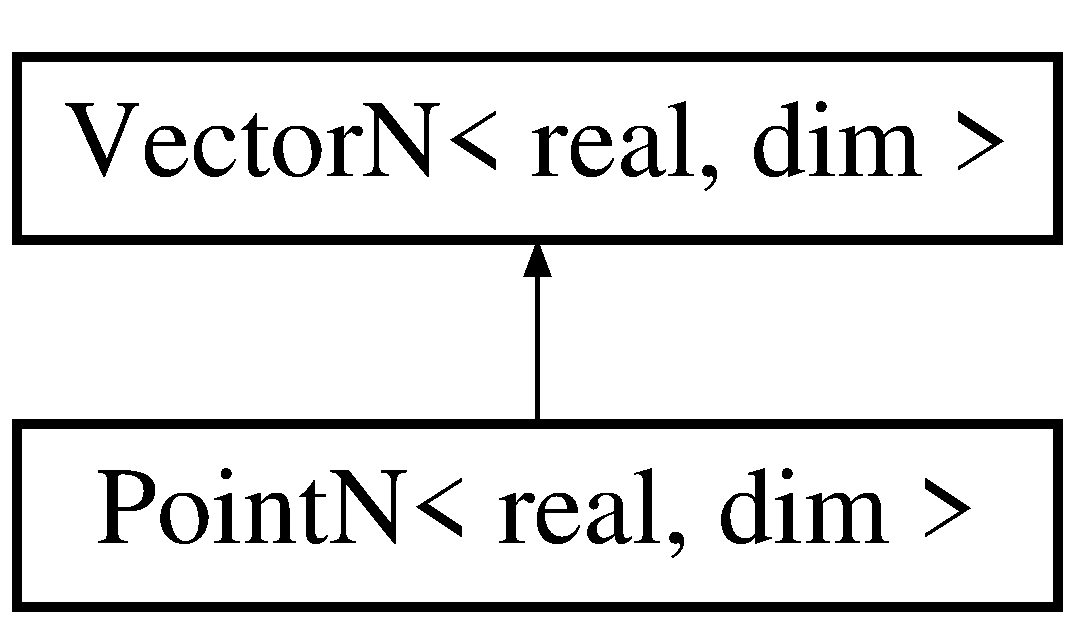
\includegraphics[height=2.000000cm]{classVectorN}
\end{center}
\end{figure}
\subsection*{Public Member Functions}
\begin{DoxyCompactItemize}
\item 
\hypertarget{classVectorN_af50158c7bc131bbfde53b5120cb6cddd}{
\hyperlink{classVectorN_af50158c7bc131bbfde53b5120cb6cddd}{VectorN} ()}
\label{classVectorN_af50158c7bc131bbfde53b5120cb6cddd}

\begin{DoxyCompactList}\small\item\em Empty constructor. \end{DoxyCompactList}\item 
\hypertarget{classVectorN_a6ef9847ef88fc72b3d0388ce79eaa2fe}{
\hyperlink{classVectorN_a6ef9847ef88fc72b3d0388ce79eaa2fe}{VectorN} (const real v\mbox{[}$\,$\mbox{]})}
\label{classVectorN_a6ef9847ef88fc72b3d0388ce79eaa2fe}

\begin{DoxyCompactList}\small\item\em Constructor from an array of coordinates. \end{DoxyCompactList}\item 
\hypertarget{classVectorN_a6dc444a7c6d3f168e0f54b5fdae51bf8}{
\hyperlink{classVectorN_a6dc444a7c6d3f168e0f54b5fdae51bf8}{VectorN} (const \hyperlink{classVectorN}{VectorN}$<$ real, dim $>$ \&v)}
\label{classVectorN_a6dc444a7c6d3f168e0f54b5fdae51bf8}

\begin{DoxyCompactList}\small\item\em Constructor from another \hyperlink{classVectorN}{VectorN}. \end{DoxyCompactList}\item 
real \& \hyperlink{classVectorN_aa926f5c408d53dfc7ec581e9b47c27ad}{operator\mbox{[}$\,$\mbox{]}} (unsigned i)
\begin{DoxyCompactList}\small\item\em Coordinate indexing. \end{DoxyCompactList}\item 
real \hyperlink{classVectorN_a5463f965a3bb96d9b2a87b6392bc15c7}{operator\mbox{[}$\,$\mbox{]}} (unsigned i) const 
\begin{DoxyCompactList}\small\item\em Coordinate indexing. \end{DoxyCompactList}\item 
bool \hyperlink{classVectorN_abdb4216ebccd9e51dc74f9f3bf5ec4eb}{operator==} (const \hyperlink{classVectorN}{VectorN}$<$ real, dim $>$ \&v) const 
\begin{DoxyCompactList}\small\item\em Equality operator. \end{DoxyCompactList}\item 
bool \hyperlink{classVectorN_a2340b63fb9299ad20b23ff162692d720}{operator!=} (const \hyperlink{classVectorN}{VectorN}$<$ real, dim $>$ \&v) const 
\begin{DoxyCompactList}\small\item\em Inequality operator. \end{DoxyCompactList}\item 
\hyperlink{classVectorN}{VectorN}$<$ real, dim $>$ \& \hyperlink{classVectorN_a7202401fb6ed378c10a06397e46d9d49}{operator=} (const \hyperlink{classVectorN}{VectorN}$<$ real, dim $>$ \&v)
\begin{DoxyCompactList}\small\item\em Assignment. \end{DoxyCompactList}\item 
\hyperlink{classVectorN}{VectorN}$<$ real, dim $>$ \& \hyperlink{classVectorN_a91138a1f8badc1c7e656005f4f7cfe30}{operator+=} (const \hyperlink{classVectorN}{VectorN}$<$ real, dim $>$ \&v)
\begin{DoxyCompactList}\small\item\em Vector sum assignment. \end{DoxyCompactList}\item 
\hyperlink{classVectorN}{VectorN}$<$ real, dim $>$ \& \hyperlink{classVectorN_a85e5e683a6f9aeff68b546ec923c737c}{operator-\/=} (const \hyperlink{classVectorN}{VectorN}$<$ real, dim $>$ \&v)
\begin{DoxyCompactList}\small\item\em Vector difference assignment. \end{DoxyCompactList}\item 
\hyperlink{classVectorN}{VectorN}$<$ real, dim $>$ \& \hyperlink{classVectorN_ab898c49e2188a964a637fdc749e9b26d}{operator$\ast$=} (real s)
\begin{DoxyCompactList}\small\item\em Multiplication by scalar assignment. \end{DoxyCompactList}\item 
\hyperlink{classVectorN}{VectorN}$<$ real, dim $>$ \& \hyperlink{classVectorN_a69839721f7fdf66ee896a91f98655274}{operator/=} (real s)
\begin{DoxyCompactList}\small\item\em Multiplication by inverse scalar assignment. \end{DoxyCompactList}\item 
\hyperlink{classVectorN}{VectorN}$<$ real, dim $>$ \hyperlink{classVectorN_a26e5f52c7b135d5d5c7775061e19647c}{operator+} (const \hyperlink{classVectorN}{VectorN}$<$ real, dim $>$ \&v) const 
\begin{DoxyCompactList}\small\item\em Vector sum. \end{DoxyCompactList}\item 
\hyperlink{classVectorN}{VectorN}$<$ real, dim $>$ \hyperlink{classVectorN_a6d4600d3a81bb8c486770771a38d6e30}{operator-\/} (const \hyperlink{classVectorN}{VectorN}$<$ real, dim $>$ \&v) const 
\begin{DoxyCompactList}\small\item\em Vector difference. \end{DoxyCompactList}\item 
{\footnotesize template$<$typename scalar $>$ }\\\hyperlink{classVectorN}{VectorN}$<$ real, dim $>$ \hyperlink{classVectorN_a829a2b55702c0fc475c3ae39d79b4e66}{operator$\ast$} (scalar s) const 
\begin{DoxyCompactList}\small\item\em Multiplication by scalar. \end{DoxyCompactList}\item 
\hyperlink{classVectorN}{VectorN}$<$ real, dim $>$ \hyperlink{classVectorN_aca314d985163785e68d412a2e73fd50c}{operator/} (real s) const 
\begin{DoxyCompactList}\small\item\em Multiplication by inverse scalar. \end{DoxyCompactList}\item 
\hyperlink{classVectorN}{VectorN}$<$ real, dim $>$ \hyperlink{classVectorN_a200e8f7a82d7681232ac18fcbd746f29}{operator-\/} () const 
\begin{DoxyCompactList}\small\item\em Symmetric operator (unary minus) \end{DoxyCompactList}\item 
real \hyperlink{classVectorN_ac969f8b5e56b59d5aef32bcde365bf24}{operator$\ast$} (const \hyperlink{classVectorN}{VectorN}$<$ real, dim $>$ \&v) const 
\begin{DoxyCompactList}\small\item\em Dot product. \end{DoxyCompactList}\item 
\hypertarget{classVectorN_abab02b195f9f65fe10b28299e5a8ccd8}{
real \hyperlink{classVectorN_abab02b195f9f65fe10b28299e5a8ccd8}{norm2} (void) const }
\label{classVectorN_abab02b195f9f65fe10b28299e5a8ccd8}

\begin{DoxyCompactList}\small\item\em Returns the square of the norm of the vector. \end{DoxyCompactList}\item 
\hypertarget{classVectorN_ae40fe34821f326f9c8ebe862c685b2b3}{
real \hyperlink{classVectorN_ae40fe34821f326f9c8ebe862c685b2b3}{norm} (void) const }
\label{classVectorN_ae40fe34821f326f9c8ebe862c685b2b3}

\begin{DoxyCompactList}\small\item\em Returns the Euclidian norm of the vector. \end{DoxyCompactList}\item 
\hypertarget{classVectorN_af6be6194bee3d68ab71217cb83639bdc}{
real \& \hyperlink{classVectorN_af6be6194bee3d68ab71217cb83639bdc}{x} (void)}
\label{classVectorN_af6be6194bee3d68ab71217cb83639bdc}

\begin{DoxyCompactList}\small\item\em Returns a reference to the first element. \end{DoxyCompactList}\item 
\hypertarget{classVectorN_adf0a31d3c269331b655ae7eba1e3f828}{
real \hyperlink{classVectorN_adf0a31d3c269331b655ae7eba1e3f828}{x} (void) const }
\label{classVectorN_adf0a31d3c269331b655ae7eba1e3f828}

\begin{DoxyCompactList}\small\item\em Returns the value of the first coordinate. \end{DoxyCompactList}\item 
real \& \hyperlink{classVectorN_a5e4c89d57463830a33a33d4ed20b2ff7}{y} (void)
\begin{DoxyCompactList}\small\item\em The y coordinate is usually the second coordinate. \end{DoxyCompactList}\item 
real \hyperlink{classVectorN_a8009604cc1f15e40f0f8459b16821992}{y} (void) const 
\begin{DoxyCompactList}\small\item\em Returns a reference to the second coordinate. \end{DoxyCompactList}\item 
real \& \hyperlink{classVectorN_acd1728a98fc3acbd47f0bcb29e542e28}{z} (void)
\begin{DoxyCompactList}\small\item\em The z coordinate is usually the third coordinate. \end{DoxyCompactList}\item 
real \hyperlink{classVectorN_a869ec216cbaba126966a10a93f5bcb0a}{z} (void) const 
\begin{DoxyCompactList}\small\item\em Returns the value of the third coordinate. \end{DoxyCompactList}\end{DoxyCompactItemize}
\subsection*{Protected Attributes}
\begin{DoxyCompactItemize}
\item 
\hypertarget{classVectorN_acf9b4d0e9c4591dd61dd0273c6b153f1}{
real \hyperlink{classVectorN_acf9b4d0e9c4591dd61dd0273c6b153f1}{coord} \mbox{[}dim\mbox{]}}
\label{classVectorN_acf9b4d0e9c4591dd61dd0273c6b153f1}

\begin{DoxyCompactList}\small\item\em Where the coordinates are actually stored. \end{DoxyCompactList}\end{DoxyCompactItemize}


\subsection{Detailed Description}
\subsubsection*{template$<$typename real = double, unsigned int dim = 3$>$class VectorN$<$ real, dim $>$}

A N-\/dimensional Vector class. 

\subsection{Member Function Documentation}
\hypertarget{classVectorN_a2340b63fb9299ad20b23ff162692d720}{
\index{VectorN@{VectorN}!operator!=@{operator!=}}
\index{operator!=@{operator!=}!VectorN@{VectorN}}
\subsubsection[{operator!=}]{\setlength{\rightskip}{0pt plus 5cm}template$<$typename real = double, unsigned int dim = 3$>$ bool {\bf VectorN}$<$ real, dim $>$::operator!= (
\begin{DoxyParamCaption}
\item[{const {\bf VectorN}$<$ real, dim $>$ \&}]{v}
\end{DoxyParamCaption}
) const\hspace{0.3cm}{\ttfamily  \mbox{[}inline\mbox{]}}}}
\label{classVectorN_a2340b63fb9299ad20b23ff162692d720}


Inequality operator. 


\begin{DoxyParams}{Parameters}
{\em v} & another vector \\
\hline
\end{DoxyParams}
\begin{DoxyReturn}{Returns}
whether this and v have at least one distinct coordinate within the error margin 
\end{DoxyReturn}
\hypertarget{classVectorN_a829a2b55702c0fc475c3ae39d79b4e66}{
\index{VectorN@{VectorN}!operator$\ast$@{operator$\ast$}}
\index{operator$\ast$@{operator$\ast$}!VectorN@{VectorN}}
\subsubsection[{operator$\ast$}]{\setlength{\rightskip}{0pt plus 5cm}template$<$typename real = double, unsigned int dim = 3$>$ template$<$typename scalar $>$ {\bf VectorN}$<$real,dim$>$ {\bf VectorN}$<$ real, dim $>$::operator$\ast$ (
\begin{DoxyParamCaption}
\item[{scalar}]{s}
\end{DoxyParamCaption}
) const\hspace{0.3cm}{\ttfamily  \mbox{[}inline\mbox{]}}}}
\label{classVectorN_a829a2b55702c0fc475c3ae39d79b4e66}


Multiplication by scalar. 


\begin{DoxyParams}{Parameters}
{\em s} & scalar \\
\hline
\end{DoxyParams}
\begin{DoxyReturn}{Returns}
product vector 
\end{DoxyReturn}
\hypertarget{classVectorN_ac969f8b5e56b59d5aef32bcde365bf24}{
\index{VectorN@{VectorN}!operator$\ast$@{operator$\ast$}}
\index{operator$\ast$@{operator$\ast$}!VectorN@{VectorN}}
\subsubsection[{operator$\ast$}]{\setlength{\rightskip}{0pt plus 5cm}template$<$typename real = double, unsigned int dim = 3$>$ real {\bf VectorN}$<$ real, dim $>$::operator$\ast$ (
\begin{DoxyParamCaption}
\item[{const {\bf VectorN}$<$ real, dim $>$ \&}]{v}
\end{DoxyParamCaption}
) const\hspace{0.3cm}{\ttfamily  \mbox{[}inline\mbox{]}}}}
\label{classVectorN_ac969f8b5e56b59d5aef32bcde365bf24}


Dot product. 


\begin{DoxyParams}{Parameters}
{\em v,:} & another vector \\
\hline
\end{DoxyParams}
\begin{DoxyReturn}{Returns}
: dot product 
\end{DoxyReturn}
\hypertarget{classVectorN_ab898c49e2188a964a637fdc749e9b26d}{
\index{VectorN@{VectorN}!operator$\ast$=@{operator$\ast$=}}
\index{operator$\ast$=@{operator$\ast$=}!VectorN@{VectorN}}
\subsubsection[{operator$\ast$=}]{\setlength{\rightskip}{0pt plus 5cm}template$<$typename real = double, unsigned int dim = 3$>$ {\bf VectorN}$<$real,dim$>$\& {\bf VectorN}$<$ real, dim $>$::operator$\ast$= (
\begin{DoxyParamCaption}
\item[{real}]{s}
\end{DoxyParamCaption}
)\hspace{0.3cm}{\ttfamily  \mbox{[}inline\mbox{]}}}}
\label{classVectorN_ab898c49e2188a964a637fdc749e9b26d}


Multiplication by scalar assignment. 


\begin{DoxyParams}{Parameters}
{\em s} & scalar \\
\hline
\end{DoxyParams}
\begin{DoxyReturn}{Returns}
reference to this (altered) vector 
\end{DoxyReturn}
\hypertarget{classVectorN_a26e5f52c7b135d5d5c7775061e19647c}{
\index{VectorN@{VectorN}!operator+@{operator+}}
\index{operator+@{operator+}!VectorN@{VectorN}}
\subsubsection[{operator+}]{\setlength{\rightskip}{0pt plus 5cm}template$<$typename real = double, unsigned int dim = 3$>$ {\bf VectorN}$<$real,dim$>$ {\bf VectorN}$<$ real, dim $>$::operator+ (
\begin{DoxyParamCaption}
\item[{const {\bf VectorN}$<$ real, dim $>$ \&}]{v}
\end{DoxyParamCaption}
) const\hspace{0.3cm}{\ttfamily  \mbox{[}inline\mbox{]}}}}
\label{classVectorN_a26e5f52c7b135d5d5c7775061e19647c}


Vector sum. 


\begin{DoxyParams}{Parameters}
{\em v} & another vector \\
\hline
\end{DoxyParams}
\begin{DoxyReturn}{Returns}
sum vector 
\end{DoxyReturn}
\hypertarget{classVectorN_a91138a1f8badc1c7e656005f4f7cfe30}{
\index{VectorN@{VectorN}!operator+=@{operator+=}}
\index{operator+=@{operator+=}!VectorN@{VectorN}}
\subsubsection[{operator+=}]{\setlength{\rightskip}{0pt plus 5cm}template$<$typename real = double, unsigned int dim = 3$>$ {\bf VectorN}$<$real,dim$>$\& {\bf VectorN}$<$ real, dim $>$::operator+= (
\begin{DoxyParamCaption}
\item[{const {\bf VectorN}$<$ real, dim $>$ \&}]{v}
\end{DoxyParamCaption}
)\hspace{0.3cm}{\ttfamily  \mbox{[}inline\mbox{]}}}}
\label{classVectorN_a91138a1f8badc1c7e656005f4f7cfe30}


Vector sum assignment. 


\begin{DoxyParams}{Parameters}
{\em v} & another vector \\
\hline
\end{DoxyParams}
\begin{DoxyReturn}{Returns}
reference to this (altered) vector 
\end{DoxyReturn}
\hypertarget{classVectorN_a6d4600d3a81bb8c486770771a38d6e30}{
\index{VectorN@{VectorN}!operator-\/@{operator-\/}}
\index{operator-\/@{operator-\/}!VectorN@{VectorN}}
\subsubsection[{operator-\/}]{\setlength{\rightskip}{0pt plus 5cm}template$<$typename real = double, unsigned int dim = 3$>$ {\bf VectorN}$<$real,dim$>$ {\bf VectorN}$<$ real, dim $>$::operator-\/ (
\begin{DoxyParamCaption}
\item[{const {\bf VectorN}$<$ real, dim $>$ \&}]{v}
\end{DoxyParamCaption}
) const\hspace{0.3cm}{\ttfamily  \mbox{[}inline\mbox{]}}}}
\label{classVectorN_a6d4600d3a81bb8c486770771a38d6e30}


Vector difference. 


\begin{DoxyParams}{Parameters}
{\em v} & another vector \\
\hline
\end{DoxyParams}
\begin{DoxyReturn}{Returns}
difference vector 
\end{DoxyReturn}
\hypertarget{classVectorN_a200e8f7a82d7681232ac18fcbd746f29}{
\index{VectorN@{VectorN}!operator-\/@{operator-\/}}
\index{operator-\/@{operator-\/}!VectorN@{VectorN}}
\subsubsection[{operator-\/}]{\setlength{\rightskip}{0pt plus 5cm}template$<$typename real = double, unsigned int dim = 3$>$ {\bf VectorN}$<$real,dim$>$ {\bf VectorN}$<$ real, dim $>$::operator-\/ (
\begin{DoxyParamCaption}
{}
\end{DoxyParamCaption}
) const\hspace{0.3cm}{\ttfamily  \mbox{[}inline\mbox{]}}}}
\label{classVectorN_a200e8f7a82d7681232ac18fcbd746f29}


Symmetric operator (unary minus) 

\begin{DoxyReturn}{Returns}
: symmetric vector 
\end{DoxyReturn}
\hypertarget{classVectorN_a85e5e683a6f9aeff68b546ec923c737c}{
\index{VectorN@{VectorN}!operator-\/=@{operator-\/=}}
\index{operator-\/=@{operator-\/=}!VectorN@{VectorN}}
\subsubsection[{operator-\/=}]{\setlength{\rightskip}{0pt plus 5cm}template$<$typename real = double, unsigned int dim = 3$>$ {\bf VectorN}$<$real,dim$>$\& {\bf VectorN}$<$ real, dim $>$::operator-\/= (
\begin{DoxyParamCaption}
\item[{const {\bf VectorN}$<$ real, dim $>$ \&}]{v}
\end{DoxyParamCaption}
)\hspace{0.3cm}{\ttfamily  \mbox{[}inline\mbox{]}}}}
\label{classVectorN_a85e5e683a6f9aeff68b546ec923c737c}


Vector difference assignment. 


\begin{DoxyParams}{Parameters}
{\em v} & another vector \\
\hline
\end{DoxyParams}
\begin{DoxyReturn}{Returns}
reference to this (altered) vector 
\end{DoxyReturn}
\hypertarget{classVectorN_aca314d985163785e68d412a2e73fd50c}{
\index{VectorN@{VectorN}!operator/@{operator/}}
\index{operator/@{operator/}!VectorN@{VectorN}}
\subsubsection[{operator/}]{\setlength{\rightskip}{0pt plus 5cm}template$<$typename real = double, unsigned int dim = 3$>$ {\bf VectorN}$<$real,dim$>$ {\bf VectorN}$<$ real, dim $>$::operator/ (
\begin{DoxyParamCaption}
\item[{real}]{s}
\end{DoxyParamCaption}
) const\hspace{0.3cm}{\ttfamily  \mbox{[}inline\mbox{]}}}}
\label{classVectorN_aca314d985163785e68d412a2e73fd50c}


Multiplication by inverse scalar. 


\begin{DoxyParams}{Parameters}
{\em s} & scalar \\
\hline
\end{DoxyParams}
\begin{DoxyReturn}{Returns}
product vector 
\end{DoxyReturn}
\hypertarget{classVectorN_a69839721f7fdf66ee896a91f98655274}{
\index{VectorN@{VectorN}!operator/=@{operator/=}}
\index{operator/=@{operator/=}!VectorN@{VectorN}}
\subsubsection[{operator/=}]{\setlength{\rightskip}{0pt plus 5cm}template$<$typename real = double, unsigned int dim = 3$>$ {\bf VectorN}$<$real,dim$>$\& {\bf VectorN}$<$ real, dim $>$::operator/= (
\begin{DoxyParamCaption}
\item[{real}]{s}
\end{DoxyParamCaption}
)\hspace{0.3cm}{\ttfamily  \mbox{[}inline\mbox{]}}}}
\label{classVectorN_a69839721f7fdf66ee896a91f98655274}


Multiplication by inverse scalar assignment. 


\begin{DoxyParams}{Parameters}
{\em s} & scalar \\
\hline
\end{DoxyParams}
\begin{DoxyReturn}{Returns}
reference to this (altered) vector 
\end{DoxyReturn}
\hypertarget{classVectorN_a7202401fb6ed378c10a06397e46d9d49}{
\index{VectorN@{VectorN}!operator=@{operator=}}
\index{operator=@{operator=}!VectorN@{VectorN}}
\subsubsection[{operator=}]{\setlength{\rightskip}{0pt plus 5cm}template$<$typename real = double, unsigned int dim = 3$>$ {\bf VectorN}$<$real,dim$>$\& {\bf VectorN}$<$ real, dim $>$::operator= (
\begin{DoxyParamCaption}
\item[{const {\bf VectorN}$<$ real, dim $>$ \&}]{v}
\end{DoxyParamCaption}
)\hspace{0.3cm}{\ttfamily  \mbox{[}inline\mbox{]}}}}
\label{classVectorN_a7202401fb6ed378c10a06397e46d9d49}


Assignment. 


\begin{DoxyParams}{Parameters}
{\em v} & another vector \\
\hline
\end{DoxyParams}
\begin{DoxyReturn}{Returns}
reference to this (altered) vector 
\end{DoxyReturn}
\hypertarget{classVectorN_abdb4216ebccd9e51dc74f9f3bf5ec4eb}{
\index{VectorN@{VectorN}!operator==@{operator==}}
\index{operator==@{operator==}!VectorN@{VectorN}}
\subsubsection[{operator==}]{\setlength{\rightskip}{0pt plus 5cm}template$<$typename real = double, unsigned int dim = 3$>$ bool {\bf VectorN}$<$ real, dim $>$::operator== (
\begin{DoxyParamCaption}
\item[{const {\bf VectorN}$<$ real, dim $>$ \&}]{v}
\end{DoxyParamCaption}
) const\hspace{0.3cm}{\ttfamily  \mbox{[}inline\mbox{]}}}}
\label{classVectorN_abdb4216ebccd9e51dc74f9f3bf5ec4eb}


Equality operator. 


\begin{DoxyParams}{Parameters}
{\em v} & another vector \\
\hline
\end{DoxyParams}
\begin{DoxyReturn}{Returns}
whether this and v have equal coordinates within the error margin 
\end{DoxyReturn}
\hypertarget{classVectorN_a5463f965a3bb96d9b2a87b6392bc15c7}{
\index{VectorN@{VectorN}!operator\mbox{[}\mbox{]}@{operator[]}}
\index{operator\mbox{[}\mbox{]}@{operator[]}!VectorN@{VectorN}}
\subsubsection[{operator[]}]{\setlength{\rightskip}{0pt plus 5cm}template$<$typename real = double, unsigned int dim = 3$>$ real {\bf VectorN}$<$ real, dim $>$::operator\mbox{[}$\,$\mbox{]} (
\begin{DoxyParamCaption}
\item[{unsigned}]{i}
\end{DoxyParamCaption}
) const\hspace{0.3cm}{\ttfamily  \mbox{[}inline\mbox{]}}}}
\label{classVectorN_a5463f965a3bb96d9b2a87b6392bc15c7}


Coordinate indexing. 


\begin{DoxyParams}{Parameters}
{\em i} & coordinate index. \\
\hline
\end{DoxyParams}
\begin{DoxyReturn}{Returns}
value of the i'th coordinate value. 
\end{DoxyReturn}
\hypertarget{classVectorN_aa926f5c408d53dfc7ec581e9b47c27ad}{
\index{VectorN@{VectorN}!operator\mbox{[}\mbox{]}@{operator[]}}
\index{operator\mbox{[}\mbox{]}@{operator[]}!VectorN@{VectorN}}
\subsubsection[{operator[]}]{\setlength{\rightskip}{0pt plus 5cm}template$<$typename real = double, unsigned int dim = 3$>$ real\& {\bf VectorN}$<$ real, dim $>$::operator\mbox{[}$\,$\mbox{]} (
\begin{DoxyParamCaption}
\item[{unsigned}]{i}
\end{DoxyParamCaption}
)\hspace{0.3cm}{\ttfamily  \mbox{[}inline\mbox{]}}}}
\label{classVectorN_aa926f5c408d53dfc7ec581e9b47c27ad}


Coordinate indexing. 


\begin{DoxyParams}{Parameters}
{\em i} & coordinate index. \\
\hline
\end{DoxyParams}
\begin{DoxyReturn}{Returns}
reference to the i'th coordinate value. 
\end{DoxyReturn}
\hypertarget{classVectorN_a8009604cc1f15e40f0f8459b16821992}{
\index{VectorN@{VectorN}!y@{y}}
\index{y@{y}!VectorN@{VectorN}}
\subsubsection[{y}]{\setlength{\rightskip}{0pt plus 5cm}template$<$typename real = double, unsigned int dim = 3$>$ real {\bf VectorN}$<$ real, dim $>$::y (
\begin{DoxyParamCaption}
\item[{void}]{}
\end{DoxyParamCaption}
) const\hspace{0.3cm}{\ttfamily  \mbox{[}inline\mbox{]}}}}
\label{classVectorN_a8009604cc1f15e40f0f8459b16821992}


Returns a reference to the second coordinate. 

Must have at least dimension 2. \hypertarget{classVectorN_a5e4c89d57463830a33a33d4ed20b2ff7}{
\index{VectorN@{VectorN}!y@{y}}
\index{y@{y}!VectorN@{VectorN}}
\subsubsection[{y}]{\setlength{\rightskip}{0pt plus 5cm}template$<$typename real = double, unsigned int dim = 3$>$ real\& {\bf VectorN}$<$ real, dim $>$::y (
\begin{DoxyParamCaption}
\item[{void}]{}
\end{DoxyParamCaption}
)\hspace{0.3cm}{\ttfamily  \mbox{[}inline\mbox{]}}}}
\label{classVectorN_a5e4c89d57463830a33a33d4ed20b2ff7}


The y coordinate is usually the second coordinate. 

Returns a reference to the second coordinate. Must have at least dimension 2. \hypertarget{classVectorN_acd1728a98fc3acbd47f0bcb29e542e28}{
\index{VectorN@{VectorN}!z@{z}}
\index{z@{z}!VectorN@{VectorN}}
\subsubsection[{z}]{\setlength{\rightskip}{0pt plus 5cm}template$<$typename real = double, unsigned int dim = 3$>$ real\& {\bf VectorN}$<$ real, dim $>$::z (
\begin{DoxyParamCaption}
\item[{void}]{}
\end{DoxyParamCaption}
)\hspace{0.3cm}{\ttfamily  \mbox{[}inline\mbox{]}}}}
\label{classVectorN_acd1728a98fc3acbd47f0bcb29e542e28}


The z coordinate is usually the third coordinate. 

Returns a reference to the third coordinate. Must have at least dimension 3. \hypertarget{classVectorN_a869ec216cbaba126966a10a93f5bcb0a}{
\index{VectorN@{VectorN}!z@{z}}
\index{z@{z}!VectorN@{VectorN}}
\subsubsection[{z}]{\setlength{\rightskip}{0pt plus 5cm}template$<$typename real = double, unsigned int dim = 3$>$ real {\bf VectorN}$<$ real, dim $>$::z (
\begin{DoxyParamCaption}
\item[{void}]{}
\end{DoxyParamCaption}
) const\hspace{0.3cm}{\ttfamily  \mbox{[}inline\mbox{]}}}}
\label{classVectorN_a869ec216cbaba126966a10a93f5bcb0a}


Returns the value of the third coordinate. 

Must have at least dimension 3. 

The documentation for this class was generated from the following file:\begin{DoxyCompactItemize}
\item 
vectorn.hpp\end{DoxyCompactItemize}

\printindex
\end{document}
